%% thesis.tex 2014/04/11
%
% Based on sample files of unknown authorship.
%
% The Current Maintainer of this work is Paul Vojta.

\documentclass[masters]{ucbmasters}
\usepackage{cite,amsmath,amssymb,amsfonts,mathrsfs,hyperref,lineno,microtype,setspace,graphicx,multicol}

\usepackage{lineno}
%\linenumbers
% Path for figures
\graphicspath{ {figures/} }

% To compile this file, run "latex thesis", then "biber thesis"
% (or "bibtex thesis", if the output from latex asks for that instead),
% and then "latex thesis" (without the quotes in each case).

% Double spacing, if you want it.  Do not use for the final copy.
% \def\dsp{\def\baselinestretch{2.0}\large\normalsize}
% \dsp

% If the Grad. Division insists that the first paragraph of a section
% be indented (like the others), then include this line:
% \usepackage{indentfirst}

\newtheorem{theorem}{Jibberish}
%\bibliographystyle{plos2015}

\begin{document}

% Declarations for Front Matter

\title{Coded Illumination Techniques for Phase Imaging and Motion Blur}
\author{Zachary F. Phillips}
\degreesemester{Fall}
\degreeyear{2016}
\degree{Master of Science}
\chair{Associate Professor Laura Waller}
\othermembers{Professor Emeritus Andrew Neureuther}
\numberofmembers{2}

\field{Applied Science and Technology}
\campus{Berkeley}

\maketitle

% Delete (or comment out) the \approvalpage line for the final version.
%\approvalpage

\copyrightpage

\begin{abstract}

Over the previous two centuries, optical microscopy has emerged as a viable tool for biological and medical research and diagnoses. Recently, the coded illumination microscope has emerged as a alternative to conventional optical systems, enabling many novel imaging techniques that are not possible with existing hardware such as quantitative phase imaging, motion deblur, and super-resolution imaging. This thesis introduces several novel coded-illumination techniques which enable phase retrieval, motion deblurring, and digital refocusing using combinations of software and hardware design. First, a single-shot quantitative phase imaging method using partially coherent color illumination is presented, enabling the synthesis of Zernike phase contrast and differential interference contrast images using a 3D-printed color filter and a color camera. This method is then further extended to motion deblurring of the linearized optical field, where we consider the imaging transfer functions in our choice of illumination pattern. Finally, a portable, smartphone-based coded-illumination microscope is presented which enables quantitative phase imaging and digital refocusing on a portable device, without the need for image post-processing on a PC. The common theme is a coded light source, which provides programmable digital contrast through the addition of a low-cost LED array. 

\end{abstract}

\begin{frontmatter}

\begin{dedication}
\null\vfil
\begin{center}
To my parents, grandparents, and sisters.
\end{center}
\vfil\null
\end{dedication}

% You can delete the \clearpage lines if you don't want these to start on
% separate pages.

\tableofcontents
%\clearpage
\listoffigures
%\clearpage
%\listoftables

\end{frontmatter}

\pagestyle{headings}

\chapter{Introduction}

\section{Optical Microscopy}

Optical microscopy is one of the oldest scientific instruments of the sciences, and continues to be an essential tool for researchers, clinicians, and engineers across many disciplines. Different from spectacles, which use a single lens to provide magnification for one or both eyes, microscopes are typically defined as having two or more refractive surfaces to provide magnification between the object of interest and the imaging plane, enabling the user to see things much smaller than the normal optical resolution of the human eye. Credit for the inventor of the compound microscope is generally attributed to Hans and Zacharias Jansen of the Netherlands, although the first published work on microscope design wasn't released until 1665 (Hooke and van Leeuwenhoek) \cite{natureMilestones,hookeMicrographica}. The term "microscope" may refer to any system which magnifies a small object for viewing using the eyes or camera. In this work, our discussion of microscopes will be limited to optical microscopes - those which are designed for use with light within the optical band of the electro-magnetic spectrum ($390nm \leq \lambda \leq 700nm$), which is approximately the electromagnetic spectrum detectable by the human eye. 

\subsection{Imaging and Resolution}
Generally speaking, a single lens may be used to form a magnified image of a sample - this is a simple consequence of the imaging condition,

\begin{equation}
\frac{1}{f} = \frac{1}{s_o} + \frac{1}{s_i}
\end{equation}

Which relates the distance of an optical element to a object under observation $s_o$ to the distance of a conjugate image $s_i$, which may be magnified by a factor $M = \frac{-s_i}{s_o}$ based on the relative distances of each quantity. The variable $f$ corresponds to the focal length of the element, which may also be an effective focal length from the combination of several refractive elements. While this optical system will magnify an object if $M > 1$, it is practically limited to smaller magnifications since there is normally a practical upper limit on $s_o$ (set by working distance) and a lower limit on the distance of the image from the lens $s_i$ (due to eyepiece design). 

The compound microscope takes advantage of multiple refractive elements to form an image. Typically, the exact number and design of these components is abstracted to the end-user, and can be defined by a relatively low number of descriptive quantities despite the complex internal lens design of a modern microscope objective. Magnification and Numerical Aperture (NA) are the most important of these physical quantities; the magnification of an objective sets the field of view which is relayed by the optic, while the numerical aperture sets a minimum bound on the resolution of the optic, often called the diffraction limit. Numerical Aperture is defined by the formula $NA=n\sin (\theta)$, where $n$ is the refractive index of the medium, and $\theta$ is the maximum half-angle at which light may pass through the objective relative to the radial (optical) axis. The angular dependance of Numerical Aperture is completely described by interference effects which arise from the wave-optics model of light propagation. As multiple off-axis sources of the same wavelength converge to a point, the wavefronts of these sources will cause constructive and destructive interference; The size of the smallest area of constructive interference is proportional to both the wavelength of the illumination and the angular separation between the two beams. Practically, the size of this spot defines the resolution of the optical system. By the Rayleigh criteria, the resolution of an optical system is set by:

\begin{equation}
\Delta x_{min}  = \frac{1.22 \lambda}{(NA_{objective} + NA_{illumination})}
\end{equation}

This Rayleigh criterion defines the minimum separation between two points which can be detected by a system with a circular aperture, and is defined by the distance between the center if the point spread function (PSF) and it's first null. This formulation combines both detection side NA ($NA_{objective}$) and illumination side NA ($NA_{illumination}$). The ratio between these NA, typically denoted as $\sigma = NA_{objective}/NA_{Illumination}$, is commonly known as the coherence factor. As $\sigma \longrightarrow 0 $, the illumination becomes spatially coherent, meaning the phase of the illumination wavefront at a given point on the sample can be perfectly defined by all other points on the sample. This definition assumes that the light source is composed of spatially distributed statistically uncorrelated emitters - normal sources such as halogen and tungsten lamps satisfy this criteria while in k{\"o}hler geometry. As sigma increases, the minimum resolvable feature size decreases, leading to images of higher quality, subject to aliasing affects. However, increasing $\sigma$ beyond 1 does not provide further resolution improvement due to the ballistic light (DC term) is not collected by the objective. This is the working principle of dark-field microscopy. Achieving resolution improvements beyond $2\times NA_{objective}$  require computational imaging techniques such as structured illumination \cite{gustafsson2000surpassing} or Fourier ptychography\cite{Zheng2013}.

\subsection{Fourier Optics Description}
The sub-field of Fourier optics provides a theoretical bridge between conventional optics and signal processing. In modern microscopes, digital cameras allow the detection of the Intensity of an optical field using a grid of photodetectors, which readily enables the use of digital signal processing techniques on images formed by a microscope. Fourier optics is especially useful for an optical system configured as a 4$f$ system:

\begin{figure}[tbh]
\centering
\includegraphics[width=0.4\textwidth]{intro-4f.png}
\caption{\label{fig:4f} Schematic of a 4$f$ optical system}
\end{figure}

In this optical configuration, the lenses in this system operate as forward and inverse Fourier Transform operators on the optical field at P1 up to a given range of support set by the NA of the lens. The Fourier Transform of P1 exists at position P2, which is often occupied by an aperture stop to limit the NA of the objective. This aperture stop prevents stray or highly abberated rays from entering the imaging plane and prevents aliasing, which is a phenomena caused by sampling a signal at a frequency which is below a the so-called Nyquist frequency, defined by the bandwidth of the measurement. In an optical system, this frequency is set by the pixel separation and system magnification relative to the imaging NA of the system. 

\section{Phase Imaging}
Visible light, like any electromagnetic (EM) radiation, is a propagating wave, and thus has both amplitude and phase. As a single coherent mode of light interacts with a general object it can be absorbed (reduced in amplitude), or reflected, refracted, or diffracted (change in phase) based on the material properties and geometry of the object. Measuring this complete electromagnetic field at the sample plane is the primary goal of an imaging system; however, current camera technology can only measure the amplitude modulation of a sample due to a finite integration time of the sensor over many periods of the arriving optical wavefront. Mathematically, this process is described as taking the magnitude of the complex field $I =|E|^2 =|Ae^{i\phi}|^2 = A^2$ where $A$ is the amplitude of a wave and $\phi$ is the phase of the wavefront in this phasor notation. Phase is related to the mechanical geometry of the cell by the relationship $\phi = \frac{2\pi}{\lambda} n d$, where $\lambda$ is the system wavelength, $n$ is the refractive index change, and $d$ is the thickness of the object.

This loss of phase information is particularly problematic for imaging aqueous samples such as cells. To counter this, biologists often apply chemical stains to add absorption contrast artificially, but this process is cumbersome and can modify the micro-environment in significant ways. Early phase imaging methods such as Differential Interference Contrast (DIC)\cite{smithDIC} and Zernike Phase Contrast (PhC) \cite{zernike1955discovered} were developed to solve this issue using interferometric tricks to mix phase and amplitude into the measurements, providing contrast for transparent specimens. These methods have since become widely adopted due to these advantages.

\section{Computational Imaging}
Computational Imaging is a recent concept which has emerged due to increasing availability of computing power and digital sensing hardware. In a Fourier optics model, an optical system can be approximated as a linear system, enabling the application of a large number of algorithms such as least squares, gradient descent, and nonlinear optimization techniques. Computational Imaging takes advantage of this mathematical description to move part of the image formation process from hardware to software. This paradigm shift enables image formation processes that were previously infeasible for conventional optical imaging, allowing an optical system designer to take advantage of the strengths of both hardware and software during each step of the image formation process.  An early example of computational imaging was the application of a cubic phase plate at the microscope pupil, which provides drastically increased depth of field but produces a highly distorted image. Since these distortions are known, however, the original image with extended depth of field can be deconvolved using knowledge of the system's point spread function (PSF)\cite{Dowski:95}. This general framework of this deconvolution problem can be represented as an inverse problem of the form:

\begin{equation}
\begin{aligned}
& \hat{x} = \underset{x}{\text{argmin}}
& & ||Ax-I ||_2^2
\end{aligned}
\end{equation}

Where $x$ represents the variable of interest (generally the object), $A$ is the forward system matrix operator, and $I$ is the measured intensity. This is the general formulation of a linear inverse problem, and is solved in various ways depending on the structure of $A$. 

In the following chapters I will describe several applications of computational imaging in optical microscopy. Chapter 2 will cover a single-shot quantitative phase imaging method which uses partially coherent color illumination to recover the complete optical field of an object from a single measurement. Chapter 3 describes an extension of this method which allows for the deblurring of an object's complete optical field as it moves across the field of view during an exposure, assuming prior knowledge of the blurring process. Chapter 4 describes Computational CellScope, a prototype device which uses a programmable domed LED illumination to perform quantitative phase imaging, digital refocusing, and multi-contrast imaging in a portable package using a smartphone for both acquisition and processing. Chapter 5 concludes this thesis and provides possible extensions of the work presented in the previous chapters.

\chapter{Single-Shot Quantitative Phase Retrieval}

\section{Quantitative Phase Imaging}
Quantitative Phase Imaging (QPI) involves recovering the amplitude and phase, or complex field, of a sample. In contrast to \emph{qualitative} phase imaging methods, such as Zernike phase contrast (PhC)\cite{zernike1955discovered}) and Differential Interference Contrast (DIC)\cite{smithDIC}, \emph{quantitative} methods recover the phase delay caused by the sample, decoupled from absorption information. Modifications of PhC~\cite{yun2010system} and DIC~\cite{CuiYangTearney2011} can make these setups quantitative, at a cost of requiring multiple images. More commonly, QPI methods use interferometry with coherent illumination and a reference beam~\cite{Popescu:06,Wang:11,Bhaduri:12}, making them expensive and sensitive to misalignment and vibrations.

Differential Phase Contrast (DPC)~\cite{Hamilton1984a,mehta2009quantitative,Tian14,tian2015quantitative} is a partially coherent QPI technique that requires multiple images. Each is captured using a different asymmetric half-circle source pattern, which shifts the sample's spectrum in Fourier space. Thus, a half circle source and its complement will cause the pupil function to crop opposite sides of the sample's spectrum. Since imaginary information is encoded in Fourier asymmetry, these images can be used to recover phase. Assuming a linearized model for a weakly scattering sample, the inverse problem becomes a single-step deconvolution process~\cite{mehta2009quantitative,tian2015quantitative}. DPC recovers both amplitude and phase with resolution up to the incoherent resolution limit ($2\times$ better than coherent methods). Practically, the illumination switching can be done quickly and at low cost with an LED array~\cite{Tian14,zijiMulti,tian2015quantitative}. At least two complementary source patterns are required, but generally 4 patterns (top, bottom, left, right half-circles) are used to avoid missing frequencies. The DPC method was recently extended to color multiplexing~\cite{lee2015color}, where the 4 source patterns were encoded into two images by using a color camera in combination with a color LED array. Similarly, color photometric stereo has been used for retrographic surface profiling of large objects using off-axis color illumination in reflection mode~\cite{johnson2009retrographic}.

Amongst the wide array of existing QPI methods, several are single-shot techniques. Off-axis holography interferes the sample beam with a tilted reference beam, then recovers phase by Fourier filtering~\cite{Witte:12}. Parallel phase-shifting can spatially multiplex several holograms within a single exposure via an array of polarizers~\cite{2004singleshotPSDH}. And single-shot QPI add-ons based on amplitude gratings work with commercial microscopes, replacing the traditional camera module~\cite{phasics,bon2012method}. Another add-on option uses two cameras to capture defocused images which can then be used to solve the Transport of Intensity Equation (TIE)~\cite{allman2005optical}. Alternatively, if chromatic aberrations are large enough, they can enable single-shot color TIE~\cite{5714248} without any hardware changes. All of these methods require the some spatial or temporal coherence, limiting resolution, but provide camera-limited frame rates.

\begin{figure}[tbh]
\centering
\includegraphics[width=\textwidth]{cdpc-Fig1.pdf}
\caption{\label{fig:hardware}
Single-shot color Differential Phase Contrast (cDPC) microscopy. a) Installation in Nikon TE300 microscope condenser turret. b) CAD model and image of fabricated cDPC insert.c) Optical schematic of a brightfield microscope with a cDPC color filter placed at the back focal plane of the condenser in K\"{o}hler configuration. d) Reconstruction: the captured color image is separated into its RGB components, which are then used to recover two unknowns (amplitude and phase) via a well-posed linear deconvolution. The sample is a micro-lens array (Fresnel Technologies 605). }
\end{figure}

\section{Color-Multiplexed Differential Phase Contrast (cDPC) }
To improve temporal resolution of a DPC system without compromising spatial resolution a multiplexing configuration is necessary to make the problem well-posed. The proposed alternative method, color Differential Phase Contrast (cDPC), requires only a \emph{single} color image for multiplexing source patterns. In this method, the source is discretized into three color channels which are used to display three different half-circle source patterns. It is important to note that while the original DPC algorithm presented in \cite{tian2015quantitative} requires 4 images, the proposed method only requires 3, since the 4th source configuration can be synthesized by taking the sum of two images acquired with opposite half-circle illuminations (a synthetic brightfield image) and subtracting that of a 90 degree rotated half-circle source. In early prototypes the color source pattern pattern was implemented in an LED array microscope, which offers many imaging modalities in one platform~\cite{Tian14,zijiMulti,tian2015quantitative,Ma:15,Phillips15, Zheng2011, Zheng2013}. However, the proposed configuration does not require a dynamic source, making it possible to use a static multi-color filter placed in the condenser back focal plane, assuming K\"{o}hler illumination. Both configurations simplify hardware and reduce costs significantly as compared to phase contrast or DIC, while providing quantitative phase, which is more general and can be used to synthesize both of the aforementioned methods digitally~\cite{JMI:JMI1027}.

\subsection{Hardware Design}
As in conventional DPC, this method requires measurements of the sample illuminated by known asymmetric sources. In cDPC, however, we make use of the microscope's existing condenser unit, which has a turret commonly used for phase contrast inserts or DIC prisms. This intermediate plane can usually be accessed easily by removing the mechanical inserts. Taking advantage of this configuration, a simple 3D printed color filter was designed and fabricated that can be placed in the condenser turret of a Nikon TE300 microscope (Figure~\ref{fig:hardware}a).

The filter prototype consists of Polyethylene Terephthalate (PET) color filters (Lee Filter, Inc.) laser cut to size and installed into a 3D printed insert designed to fit our microscope. Narrow bandwidth illumination filters (e.g. multi-layer coated glass) would separate colors better, but suffer from low light throughput and high cost. Therefore, inexpensive and easy-to-cut PET film filters were used; the resulting cross-talk between color channels will be accounted for in post-processing, described below.

The total cost of raw materials is approximately $\$30$ and filters were produced quickly with a 3D printer and laser cutter. One filter is shown in Figure~\ref{fig:hardware}b; it was installed in the condenser turret of an inverted microscope (Figure~\ref{fig:hardware}a), replacing one of the removable phase contrast (Ph1, Ph2 or Ph3) inserts.
\subsection{Calibration}
\label{Calibration}

Ideally, the color filters would provide perfect separation of the three source patterns into the three color channels. In reality, both the illumination and camera color channels have cross-talk between the desired wavelengths. To account for this, system calibration is separated into two separate steps: detection-side and illumination-side.

Illumination-side calibration corrects for the relative spectral transmittance of each of the source color filters. The illumination pattern simultaneously encodes three half-circle sources, one each for the RGB color channels. Red and green are opposite half-circles, and blue is rotated by 90 degrees relative to the others. Where the blue and green patterns overlap, a cyan filter (blue + green) was used. Where the blue and red patterns overlap, a purple filter (blue + red) was used. Hence, the final filter design actually contains four quadrants having red, green, cyan and purple filters (see Fig.~\ref{fig:transferfunctions}).

\begin{figure}[tbh]
\centering
\includegraphics[width=0.8\textwidth]{cdpc-Fig2.pdf}
\caption{\label{fig:transferfunctions}
Transfer functions for amplitude and phase contrast in each cDPC color channel. Left: Spectral contribution of each illumination filter as captured by the camera's Bayer pattern. The following columns show the components of the amplitude and phase transfer functions in the spatial frequency domain and the source represented in each image.  Bottom row: sum of each column, representing the calibrated and scaled source and the total coverage of amplitude and phase transfer functions, respectively. }
\end{figure}

When filtered by the sensor Bayer pattern, the filter spectrum bases are not orthogonal. This can be seen in the spectra of each PET film after capture with a color camera (left column of Fig.~\ref{fig:transferfunctions}). The result is an undesirable loss of asymmetry in the source that reduces phase SNR. However, it is possible to account for the asymmetry during reconstruction by modeling the source patterns as in Fig.~\ref{fig:transferfunctions}.

Detection-side calibration accounts for spectral cross-talk of the camera color channels. Standard RGB Bayer filters do not provide perfect discrimination between RGB wavelengths, but coupling artifacts can be removed by calibration. Given the pixel values from the raw color image with an RGBG Bayer filter ($I_r$, $I_{g1}$, $I_{g2}$, $I_b$), it is possible to solve for the decoupled color image ($I_R$, $I_{G}$, $I_{B}$) that would be obtained if the sample were illuminated with a single color, according to the following equation,

\begin{equation}
\label{eq:couplingmatrix}
\begin{bmatrix}
I_{r} \\
I_{g1}\\
I_{g2}\\
I_{b}
\end{bmatrix}
 =
 C
 \begin{bmatrix}
I_{R} \\
I_{G}\\
I_{B}
\end{bmatrix}.
\end{equation}

\noindent  The matrix $C$ is a 4$\times$3 calibration matrix describing the coupling between each color channel. It is generated by filtering the broadband source with each filter independently, then measuring the relative red ($I_R$), green ($I_G$) and blue ($I_B$) read-outs to populate the corresponding column vectors of the $C$ matrix. The ratio between the intensities of each flat-field image at each detection channel provides a linear weighting of the contribution of each source to the color measurement. Once $C$ has been measured once, it can be used to pre-process all later measurements by solving Eq.~\eqref{eq:couplingmatrix}. This step is important for reducing artifacts in the phase results.

Another important step for cDPC is to account for wavelength-dependent changes in phase and spatial frequency. DPC recovers absorption ($\mu$) and phase ($\phi$) information from intensity measurements. These quantities are defined as:

\begin{equation}
\label{eq:absorption_phase}
\mu = \frac{2\pi}{\lambda_0} \alpha d,\ \phi = \frac{2\pi}{\lambda_0} n d,
\end{equation}

\noindent where $\lambda_0$ is a reference wavelength, $d$ is the thickness of the sample, $n$ represents refractive index and $\alpha$ indicates absorption coefficient. Absorption and phase transfer functions are determined by illumination numerical aperture (NA), objective NA and illumination wavelength~\cite{tian2015quantitative}. In the proposed color-multiplexed DPC method, the transfer functions must also consider the change in wavelength of each color channel. Phase ($\phi$) depends on which wavelength is used. By assuming no dispersion in the sample, it is possible to use Eq.~\eqref{eq:absorption_phase} to synthesize phase for any wavelength by simply multiplying the optical path length ($nd$) by the wave number ($\frac{2\pi}{\lambda_0}$) of a desired reference wavelength $\lambda_0$.

\subsection{Forward model}
\label{sec:forward}
Here a linearized forward model is formed by deriving the Weak-Object Transfer Functions (WOTFs) for both amplitude and phase ~\cite{Claus2015, tian2015quantitative, Hamilton1984a}. The WOTF formulation linearizes phase recovery by neglecting the nonlinear scatter-scatter term; this is a good approximation when the object is weak (having low absolute phase or amplitude). Each image is modeled as the sum of convolutions between color-dependent point spread functions (PSFs) for intensity, and physical quantities - absorption and phase ($\mu$, $\phi$),

\begin{equation}
	I(\vec{r},\lambda) = I_{0}(\lambda) +H_{\mu}(\vec{r},\lambda) * \mu(\vec{r}) + \mathrm{i}\cdot H_{\phi}(\vec{r},\lambda) * \phi(\vec{r}),
	\label{eq:two}
\end{equation}

\noindent where $\vec{r}$ represents 2D real-space coordinates, $I$ is the color intensity measurement, $I_0$ is the background signal, $*$ denotes convolution, $H_{\mu}$ and $H_{\phi}$ are PSFs for absorption and phase, respectively. Taking the 2D Fourier transform of both sides of Eq.~\ref{eq:two}, we obtain:

\begin{equation}
	\tilde{I}(\vec{f},\lambda) = \tilde{I}_0(\lambda)\cdot\delta(\vec{f})+ \tilde{H}_{\mu}(\vec{f},\lambda)  \cdot \tilde{\mu}(\vec{f})+ \mathrm{i}\cdot\tilde{H}_{\phi}(\vec{f},\lambda)  \cdot \tilde{\phi}(\vec{f}),
\end{equation}

\noindent where $\vec{f}$ is 2D spatial frequency coordinates, $\tilde{\cdot}$ denotes Fourier transform,  $\tilde{H}_{\mu}$ and $\tilde{H}_{\phi}$ are the wavelength-dependent transfer functions for absorption and phase, respectively. Given a known source ($S$), and pupil function ($P$) which is modeled as a circle with radius set by the objective NA and wavelength $\lambda$, the transfer functions are~\cite{Claus2015,tian2015quantitative}:

\begin{equation}\label{WOTFre}
\tilde{H}_{\mu}(\vec{f},\lambda) = \left[  P(\vec{f},\lambda) \star (P(\vec{f},\lambda)\cdot S(-\vec{f},\lambda))+ (P(\vec{f},\lambda) \cdot S(-\vec{f},\lambda)) \star P(\vec{f},\lambda)\right]
\end{equation}

\begin{equation}\label{WOTFim}
\tilde{H}_{\phi}(\vec{f},\lambda) = \frac{\lambda_0}{\lambda}\cdot\left[ P(\vec{f},\lambda) \star (P(\vec{f},\lambda)\cdot S(-\vec{f},\lambda))- (P(\vec{f},\lambda) \cdot S(-\vec{f},\lambda)) \star P(\vec{f},\lambda) \right],
\end{equation}

\noindent where $\star$ denotes cross-correlation. Note that because spatial frequency is a function of wavelength, the source shape $S(\lambda)$ and pupil function $P(\lambda)$ also depend on wavelength. Specifically, the diameters of the source and transfer functions in Fourier space are inversely proportional to the wavelength of the color channel. Hence, blue illumination provides larger Fourier space coverage and better resolution than red. The proposed modified forward model accounts for these differences in the color channel's transfer function. Figure~\ref{fig:transferfunctions} shows the absorption and phase transfer functions for $\lambda = 450 nm$, $\lambda = 546 nm$ and $\lambda = 670 nm$, with top-right, bottom-right and top-left half-circle sources, respectively.

Examining Fig.~\ref{fig:transferfunctions}, it is clear that the absorption transfer functions for each color channel are symmetric low-pass filters. The phase transfer functions, on the other hand, are asymmetric band-pass-like filters with a line of missing frequencies along the axis of asymmetry. By rotating the blue half-circle by 90 degrees relative to the red and green ones, the missing line is filled. The overall amplitude and phase transfer functions for cDPC are shown in the last row of Fig.~\ref{fig:transferfunctions}, calculated by summing the absolute values of each color transfer function. As with previous DPC implementations, absorption information loses contrast at high spatial frequencies. Phase has a similar drop-off at high frequencies, but also loses contrast in the low spatial frequency regions. Hence, SNR will be important for accurately recovering low-frequency phase information. The maximum spatial frequency range captured is 2$\times$ the NA of the blue color channel. However, the final resolution using cDPC is set by the diffraction limit of green light, since total frequency coverage is set by the maximum spatial frequency which is measured by \textit{two or more} color channels. This comes as an implication of trying to recover two unknowns, amplitude and phase, thus requiring at least two measurements.

\subsection{Inverse problem}
Using the forward model developed in Section~\ref{sec:forward}, the cDPC inverse problem aims to minimize the difference between the measured color image and that which would be measured, given the estimate of the sample's amplitude and phase:

\begin{equation}\label{eq:objectivefunction}
\begin{split}
\min_{\mu,\phi} \sum_{m=1}^{3}\frac{1}{2} \parallel\tilde{I}'(\lambda_m) - \tilde{H}_{\mu}(\lambda_m)\cdot \tilde{\mu} - \mathrm{i}\cdot\tilde{H}_{\phi}(\lambda_m)\cdot \tilde{\phi} \parallel_2^2 + R(\mu,\phi),
\end{split}
\end{equation}

\noindent where $\tilde{I}'$ is the spatial frequency spectrum of the background-subtracted intensity, $m$ is the wavelength index and $R(\mu,\phi)$ is a regularization term (typically on the order of $10^{-3}$). This problem is linear and can be solved with a one-step least-square solution (e.g. Wiener deconvolution~\cite{HayesDSP}) or by an iterative algorithm (e.g. gradient descent). The ideal choice of regularizer $R(\mu,\phi)$ depends on the sample and noise. Basic $\ell_2$ regularization should be tuned to suppress noise amplification in spatial frequencies that are measured with low-contrast, without destroying sample information at those frequencies. Alternatively, if the sample is sparse (only a few non-zero values), one can use an $\ell_1$ regularizer~\cite{2002_l1_sparcity}. Other types of \textit{a priori} information may be incorporated by appropriate regularization. In the experiments presented here no assumptions on the sample structure were made; However, $\ell_2$ regularization is used to constrain the total energy of the signal and make the problem well-posed. Equation~\eqref{eq:objectivefunction} thus becomes,

\begin{equation}\label{eq:objectivefunction2}
\begin{split}
\min_{\mu,\phi} \sum_{m=1}^{3} \frac{1}{2}  \parallel\tilde{I}'(\lambda_m) - \tilde{H}_{\mu}(\lambda_m)\cdot \tilde{\mu} - \mathrm{i}\cdot\tilde{H}_{\phi}(\lambda_m)\cdot \tilde{\phi} \parallel_2^2 + \gamma_\mu\cdot \parallel \mu\parallel^2_2 + \gamma_\phi\cdot \parallel \phi\parallel^2_2,
\end{split}
\end{equation}

\noindent which remains differentiable and allows us to find the global minimum solution for absorption and phase with a single matrix inversion step. The final reconstruction for the absorption and phase maps can therefore be written mathematically as:

\begin{equation} \label{eq:Ha}
\mu = F^{-1}\left\{\frac{\left(\sum\limits_{m}|\tilde{H}_{\phi,m}|^2+\gamma_{\phi}\right)\cdot\sum\limits_{m}\left(\tilde{H}^*_{\mu,m}\cdot\tilde{I}'_{m}\right)-\sum\limits_{m} \left ( \tilde{H}^*_{\mu,m}\cdot\tilde{H}_{\phi,m} \right ) \cdot\sum\limits_{m}\left(\tilde{H}^*_{\phi,m}\cdot\tilde{I}'_{m}\right)}{\left(\sum\limits_{m}|\tilde{H}_{\mu,m}|^2+\gamma_{\mu}\right)\cdot\left(\sum\limits_{m}|\tilde{H}_{\phi,m}|^2+\gamma_{\phi}\right) - \sum\limits_{m}\left(\tilde{H}_{\mu,m}\cdot\tilde{H}^*_{\phi,m}\right)\cdot\sum\limits_{m}\left(\tilde{H}^*_{\mu,m}\cdot\tilde{H}_{\phi,m}\right)} \right\}
\end{equation}

\begin{equation} \label{eq:Hp}
\phi = F^{-1}\left\{\frac{-\mathrm{i}\cdot\left[\left(\sum\limits_{m}|\tilde{H}_{\mu,m}|^2+\gamma_{\mu}\right)\cdot\sum\limits_{m}\left(\tilde{H}^*_{\phi,m}\cdot\tilde{I}'_{m}\right)-\sum\limits_{m}\left(\tilde{H}_{\mu,m}\cdot\tilde{H}^*_{\phi,m}\right)\cdot\sum\limits_{m}\left(\tilde{H}^*_{\mu,m}\cdot\tilde{I}'_{m}\right)\right]}{\left(\sum\limits_{m}|\tilde{H}_{\mu,m}|^2+\gamma_{\mu}\right)\cdot\left(\sum\limits_{m}|\tilde{H}_{\phi,m}|^2+\gamma_{\phi}\right)-\sum\limits_{m}\left(\tilde{H}_{\mu,m}\cdot\tilde{H}^*_{\phi,m}\right)\cdot\sum\limits_{m} \left( \tilde{H}^*_{\mu,m}\cdot\tilde{H}_{\phi,m} \right )} \right\},
\end{equation}

\noindent where $\cdot$ represents point-wise matrix multiplication, $\gamma_\mu$ and $\gamma_\phi$ are regularization coefficients of absorption and phase, respectively, and $F^{-1}$ denotes the inverse DFT operation. To compute amplitude ($A$) from absorption, the relation $A = e^{\mu}$, is used, which is similar to the reconstruction method used in~\cite{tian2015quantitative} but does not assume a pure phase object, leading to additional terms in Eq.~\ref{eq:Hp}.

\begin{figure}[bth]
\centering
\includegraphics[width=\textwidth]{cdpc-Fig3.pdf}
\caption{\label{fig:spatialRes}
Experimental comparison of single-shot cDPC with monochromatic DPC and through-focus phase retrieval methods. (Left) Source patterns. (Middle) Raw camera measurements. (Right) Recovered optical field. DPC methods (partially coherent) were acquired using a 20$\times$ 0.4 NA objective lens, while through-focus images (spatially coherent) were captured using 60$\times$ 0.8 NA, in order to ensure equal resolution in all cases.}
\end{figure}

\clearpage

\section{Validation}

To experimentally validate the proposed cDPC method, results were compared with two established QPI methods: monochromatic DPC and through-focus phase retrieval (Fig.~\ref{fig:spatialRes}). For fair comparison, all are implemented on the same Nikon TE300 microscope using illumination generated by an RGB LED array (Adafruit). Each cDPC experiment uses a discretized version of the cDPC color filter design displayed on the LED array. Monochromatic DPC uses 4 images captured with each of 4 asymmetric source patterns~\cite{zijiMulti}. Through-focus phase imaging uses only the central green LED (for temporal and spatial coherence) while capturing 14 images at different focus depths; phase is then recovered by a nonlinear optimization phase retrieval method~\cite{JingsanSourceRecovery2016}.

Because of the coherent illumination, through-focus phase imaging has 2$\times$ worse resolution than DPC methods. Thus, a 20$\times$ 0.4 NA objective lens was used for DPC methods, but switched to a 60$\times$ 0.8 NA objective for through-focus phase, in order keep resolution equal for all three. Spatial resolution is quantified using a spoke-pattern phase target~\cite{standardphaseresolution2016}.

As can be seen in Fig.~\ref{fig:spatialRes}, the RGB color channel images have similar contrast to the left, right and top images of the monochromatic DPC, as expected. The phase results are also similar, with equivalent spatial resolution. Because the cDPC image is captured in one shot with color filters, it has lower SNR than monochromatic DPC and deviates in its low-frequency fluctuations, which have weaker transfer function values. Overall, however, single-shot cDPC performs comparably to multi-shot DPC.

Next, the LED array was removed and replaced with the existing illumination pathway. For illumination, a broadband arc lamp light source was used. Alternatively, a high-power blue-phosphor static LED source could be used. The color filter insert shown in Fig.~\ref{fig:hardware}b was then installed into the condenser turret. Figure~\ref{fig:mosaic} shows amplitude and phase reconstructions from the proposed cDPC method with objectives of various magnification. The cDPC method is compatible with any standard objective having $ NA_{objective}\leq NA_{condenser}$. If an objective with larger NA than the condenser NA is used, the low frequencies of phase will not be transmitted during image formation (see the phase transfer function in Fig. \ref{fig:transferfunctions}), since phase contrast comes primarily from high-angle illumination. The spatial coherence factor $\sigma$ is often defined as:

\begin{equation}
\sigma = \frac{NA_{condenser}}{NA_{objective}}.
\end{equation}

\noindent In other words, $\sigma < 1$ will result in reduced phase contrast as compared to the $\sigma \geq 1$ case. The Nikon TE300 microscope used in this study was configured with a 0.53 NA condenser lens. Imaging with a higher objective NA would require high-NA illumination (e.g. by using a domed LED array~\cite{Phillips15}). Temporal coherence is set by the bandwidth of the color filters, since these have narrower bandwidth than the camera filters. The full-width-half-maximum (FWHM) bandwidth for the filters used in this study was approximately 50nm, which is similar to the emission spectrum of the LED array used previously~\cite{tian2015quantitative}.

\begin{figure}[ph]
\centering
\includegraphics[width=1\textwidth]{cdpc-Fig4.pdf}
\caption{\label{fig:mosaic}
Phase and amplitude reconstructions for various samples and magnifications. (First column) Micro-lens array, 4x 0.1 NA. (Second column) Wild-type c. elegans, 10x 0.25 NA. (Third column) HEK 293T cells, 20$\times$ 0.4 NA). (Fourth column) MCF7 cells, 20$\times$ 0.4 NA.}
\end{figure}

\clearpage


\subsection{Temporal Resolution}
Since cDPC is single-shot, temporal resolution is set by the camera's frame rate, giving a factor of 4 improvement over conventional DPC. Single-shot methods reduce artifacts due to motion blur and image registration. This can be seen in Fig.~\ref{fig:temporalRes}, where the performance cDPC and conventional DPC are compared when imaging a live c. elegans culture. Motion blur is significantly reduced with cDPC, since the sample changes rapidly between frames, even at 12.5 frames per second.

\begin{figure}[tbh]
\centering
\includegraphics[width=\textwidth]{cdpc-Fig5.pdf}
\caption{\label{fig:temporalRes}
Experimental demonstration of motion blur reduction with cDPC vs. conventional DPC. The cDPC method results in significantly reduced motion blur artifacts due to its single-shot acquisition.}
\end{figure}

\subsection{Synthesized PhC and DIC Images}

\begin{figure}[tbh]
\centering
\includegraphics[width=\textwidth]{cdpc-Fig6.pdf}
\caption{\label{fig:synthDIC_PC}
Comparison of standard DIC and PhC images to their synthesized counterparts from cDPC. Ground truth DIC images were acquired using a 20x 0.75 NA objective and phase contrast images using a 20x 0.4 NA PhC objective. cDPC images were acquired using a 20x 0.4 NA objective and the filter insert.}\end{figure}

Differential Interference Contrast (DIC) and conventional Phase Contrast (PhC) microscopy are examples of the widespread adoption of phase imaging methods in medicine and biomedical research. Though both methods have gained widespread adoption, optical components required for their implementation remain expensive, and alignment by an experienced user is required for acceptable performance. Both DIC and phase contrast can be described by forward models which produce a qualitative mixture of amplitude and phase images~\cite{zernike1942phase, smithDIC}. Since the forward models of these systems are well known, quantitative phase imaging methods can be used to form these images digitally, mimicking the physical optical system through numerical simulation. Synthesized images from cDPC, as well as ground truth DIC and PhC images, are shown in Figure~\ref{fig:synthDIC_PC} to be comparable.

Synthesizing DIC and PhC is of particular use for clinicians and researchers who have been trained to make diagnoses or decisions based on these images. While all QPI methods can be used to synthesize these images, the cDPC method is particularly well-suited since it is single-shot, allowing for real-time digital synthesis. In addition, cDPC is much cheaper to implement than either DIC or PhC, since it requires only the addition of an inexpensive color filter insert and no specialized objectives. In contrast, DIC prisms and phase contrast objectives (specific to a given NA) can drive up the cost of a microscope significantly.

\subsection{Stained and Dispersive Samples}
The cDPC method uses color multiplexing to recover complex-field, making an inherent assumption that the sample is both non-dispersive and colorless. Non-dispersive means that the refractive index does not change appreciably with wavelength:

\begin{equation} \label{Eq:nonDispersive}
\phi(n(\lambda),d,\lambda) \approx \phi(n_0,d,\lambda).
\end{equation}

\noindent This assumption implies that the optical path length ($OPL = nd$) will remain constant for all measurements. The relative phase delay will always vary with $\lambda$ (Eq. \ref{eq:absorption_phase}), but this is accounted for in the cDPC algorithm by scaling the transfer functions based on the relative wavelength of each color channel. Unless the dispersion curve is known and the material is assumed to be uniform, one cannot account for dispersive effects in the sample using the proposed algorithm. However, in practice these effects do not corrupt our phase reconstructions results significantly due to relatively small dispersive effects of water across optical wavelengths.

The second assumption is that the sample is colorless, meaning that the absorption does not have chromatic dependence:
\begin{equation} \label{outEq:monochrome}
\mu(\lambda) \approx \mu_0.
\end{equation}
\noindent This is generally valid for unstained biological samples, which are transparent. Color variations due to filter transmission coefficients at different wavelengths are present, but can be removed by the calibration procedure described in Section 1.2. Color-dependent absorption, such as that created by stained samples, cannot be recovered and will cause errors in the phase result. In practice, these assumptions limit the applicability of the cDPC method to unstained uncolored samples. However, quantitative phase reveals the mechanical structure of the microenvironment with high contrast, which may eliminate the need for staining in many applications.

% \chapter{Motion Deblurring using Partially-Coherent Coded Illumination}

\section{High-Throughput Imaging}
Throughput is a primary concern for many imaging applications - for example, the clinical laboratory a large hospital may need to scan hundreds of histology slides per hour. Often, slide imaging or scanning large samples at high resolution requires the registration and tiling of many images acquired using a high-magnification objective. The acquisition of these datasets is often very long, owing to the precise positioning required as well as a necessary autofocusing step prior to each acquisition. Optimization of this process would clearly benefit hospitals and research centers studying datasets which necessitate a large field of view with high resolution.

Most modern high-throughput imaging systems use a stop-and-stare imaging style, where images are acquired by moving the sample to many positions, stopping, autofocusing, and finally acquiring an image. The full-field image is then stitched together using a registration algorithm. As mentioned previously, this method is often prohibitively slow due to the time necessary to stop and start the motion as well as autofocusing. A promising alternative to this scheme is strobed illumination, where the sample is moved constantly while the illumination is strobed, or flashed once each exposure using a very short, high-intensity pulse width. In this framework the image is still blurred, but the blurring is designed to be smaller than the system PSF causing no image degradation.

\section{Motion Deblur}

Strobed illumination is an ideal implementation in many applications. However, producing a very bright, very short pulse can often be difficult, particularly when a sample is moving fast, or in a low-resource setting such as a portable device where illumination power and intensity are restrcted. A promising alternative to strobed illumination is motion compensation using a deblurring algorithm which incorporates hardware coding techniques. Non-blind motion deblurring was previously explored in the context of computational photography, including several hardware implementations which exploit multiple cameras \cite{nayarDeblur, CaiDeblurring} or coded exposures \cite{raskar2006coded}. In addition, blind deblurring for photography has been extensively studied in the context of computational photography, where priors such as object statistics \cite{fergus2006removing, Shan:2008:HMD:1360612.1360672,Cho:2009:FMD:1618452.1618491,levin2006blind} and wavelet sparsity \cite{caiWavelet} to solve for the blur kernel and latent image simultaneously. In general, in-plane motion blur can be modeled as the convolution of a static intensity image ($I_s$) with a blur kernel $B$, which defines the smearing of a single point as it is moved across the field of view during a single exposure:

\begin{equation}\label{blurForwardModel}
I_{blurred}  (\vec{r})= I_0(\vec{r}) *  B(\vec{r})
\end{equation}

Here $\vec{r}$ and $\vec{k}$ represent the spatial coordinates and the Fourier conjugate variables for k-space respectively, and $I_0$ is the unblurred image of the sample or scene. In this simple case, we assume complete knowledge of the blur kernel $B$. The inverse problem can be formulated as a simple deconvolution of the static intensity image:

\begin{equation}\label{eq:blurInverseModel}
\tilde I_0 (\vec{r}) = \mathscr{F}^{-1}_{2D} \{\frac{I_{blurred}}{ \tilde{B}(\vec{k})}\}
\end{equation}

Where $\tilde{\cdot}$ denotes the 2D Fourier Transform. This inverse problem is a standard deconvolution problem and can be solved using a single least squares operation. Like most deconvolution problems, this problem is ill-posed and requires regularization to solve due to small values or zeros in the spectrum of $B$. This regularizer can be tailored to the problem using a-priori information about the sample, but in general a $\ell_2$ regularizer provides adequate results, and allows a single-step solution for a general object.

In many cases we not only know $B$ a priori, but have complete control over the shape of $B$ subject to practical hardware constraints. We can, therefore, choose an optimal motion pathway as well as illumination or exposure magnitude before acquiring to enhance the quality of our reconstructions. In the case where exposure is not coded, $B$ is simply a 1D \textit{rect} function placed into a 2D image as shown in Fig. \ref{fig:deblur}. In the Fourier domain, this transforms to a \textit{sinc} function, which has many zero crossings, making it hard to invert even if $B$ is perfectly known. The problem of designing an optimal $B$ motivated the design of the flutter-shutter camera \cite{raskar2006coded}. In this design, a ferrite shutter was placed in front of a camera lens and was opened and closed repeatedly during a single camera exposure. As a sample moves across the field it is convolved with this shutter time series, mapped to the spatial dimension by the velocity of the object, which is assumed to be known. This allows the user to optimize the blur kernel based on the object's velocity and exposure time.

A common metric for the fitness of a particular choice of $B$ is the condition number $\kappa$.  Generally, the condition number is the ratio of the larges to smallest singular value of the filter $H$. For linear shift-invariant (LSI) systems these are equal to the absolute value of the maximum and minimum Fourier coefficients respectively:

\begin{equation}\label{condNum}
 \kappa\{B\} = \frac{\sigma_{max}\{B\}}{\sigma_{min}\{B\}} = ||B||_p || B^{-1}||_p = \frac{\max{|\tilde{B}(\vec{k})|}}{\min{|\tilde{B}(\vec{k})|}}
\end{equation}

This metric can be evaluated quickly which makes optimizing $B$ directly numerically feasible. Essentially, this metric promotes a flat Fourier spectrum of $B$ and penalizes values close to zero, which makes the problem well-posed. It is important to note that the optimum solution of $B$ is clearly a delta function $\delta(\vec{r})$, and this optimization will converge to this solution if left unconstrained. However, a delta function corresponds to strobed illumination, which provides much less overall exposure, and therefore a much noisier image compared to constant exposure. To counter this, we place a box constraint on the maximum intensity of the illumination, which has practical motivations based on the maximum illumination intensity. In practice we bound $B\in[0,1]$. In addition we place a constraint on the total illumination throughput of the system during an exposure time, $\sum_{\vec{r}} B(\vec{r})\geq \gamma$, where $\gamma$ is typically set to 50$\%$ of the maximum intensity to allow the algorithm reasonable freedom as in \cite{raskar2006coded}. The complete problem is expressed as:

\begin{equation}
\label{eq:deblurKernelProb}
\begin{aligned}
& \underset{B}{\text{minimize}}
& & \kappa \{ B \} = \frac{\max{|\tilde{B}(\vec{k})|}}{\min{|\tilde{B}(\vec{k})|}} \\
& \text{subject to}
& & \sum_{n=1}^N B[n] \geq \gamma N, \hspace{15pt} 0 \leq B[n] \leq 1 \hspace{5pt} \forall n
\end{aligned}
\end{equation}


Figure \ref{fig:deblur} shows example blur kernels with their representations in real space and Fourier space. Noise also plays an important role, as noise will corrupt spatial frequencies which have poor transmission, further motivating the design of kernels with a flat Fourier spectrum. This method was also applied to microscopy using programmable LED array illumination which allows motion deblurring by varying the intensities of the LED array during exposure times \cite{Ma:15}. Unlike the ferro-electric shutter used in \cite{raskar2006coded}, the LED array has no moving parts, which allows faster update speeds, and can provide coded multi-color illumination if tri-color LEDs are used.


\begin{figure}[ph]
\centering
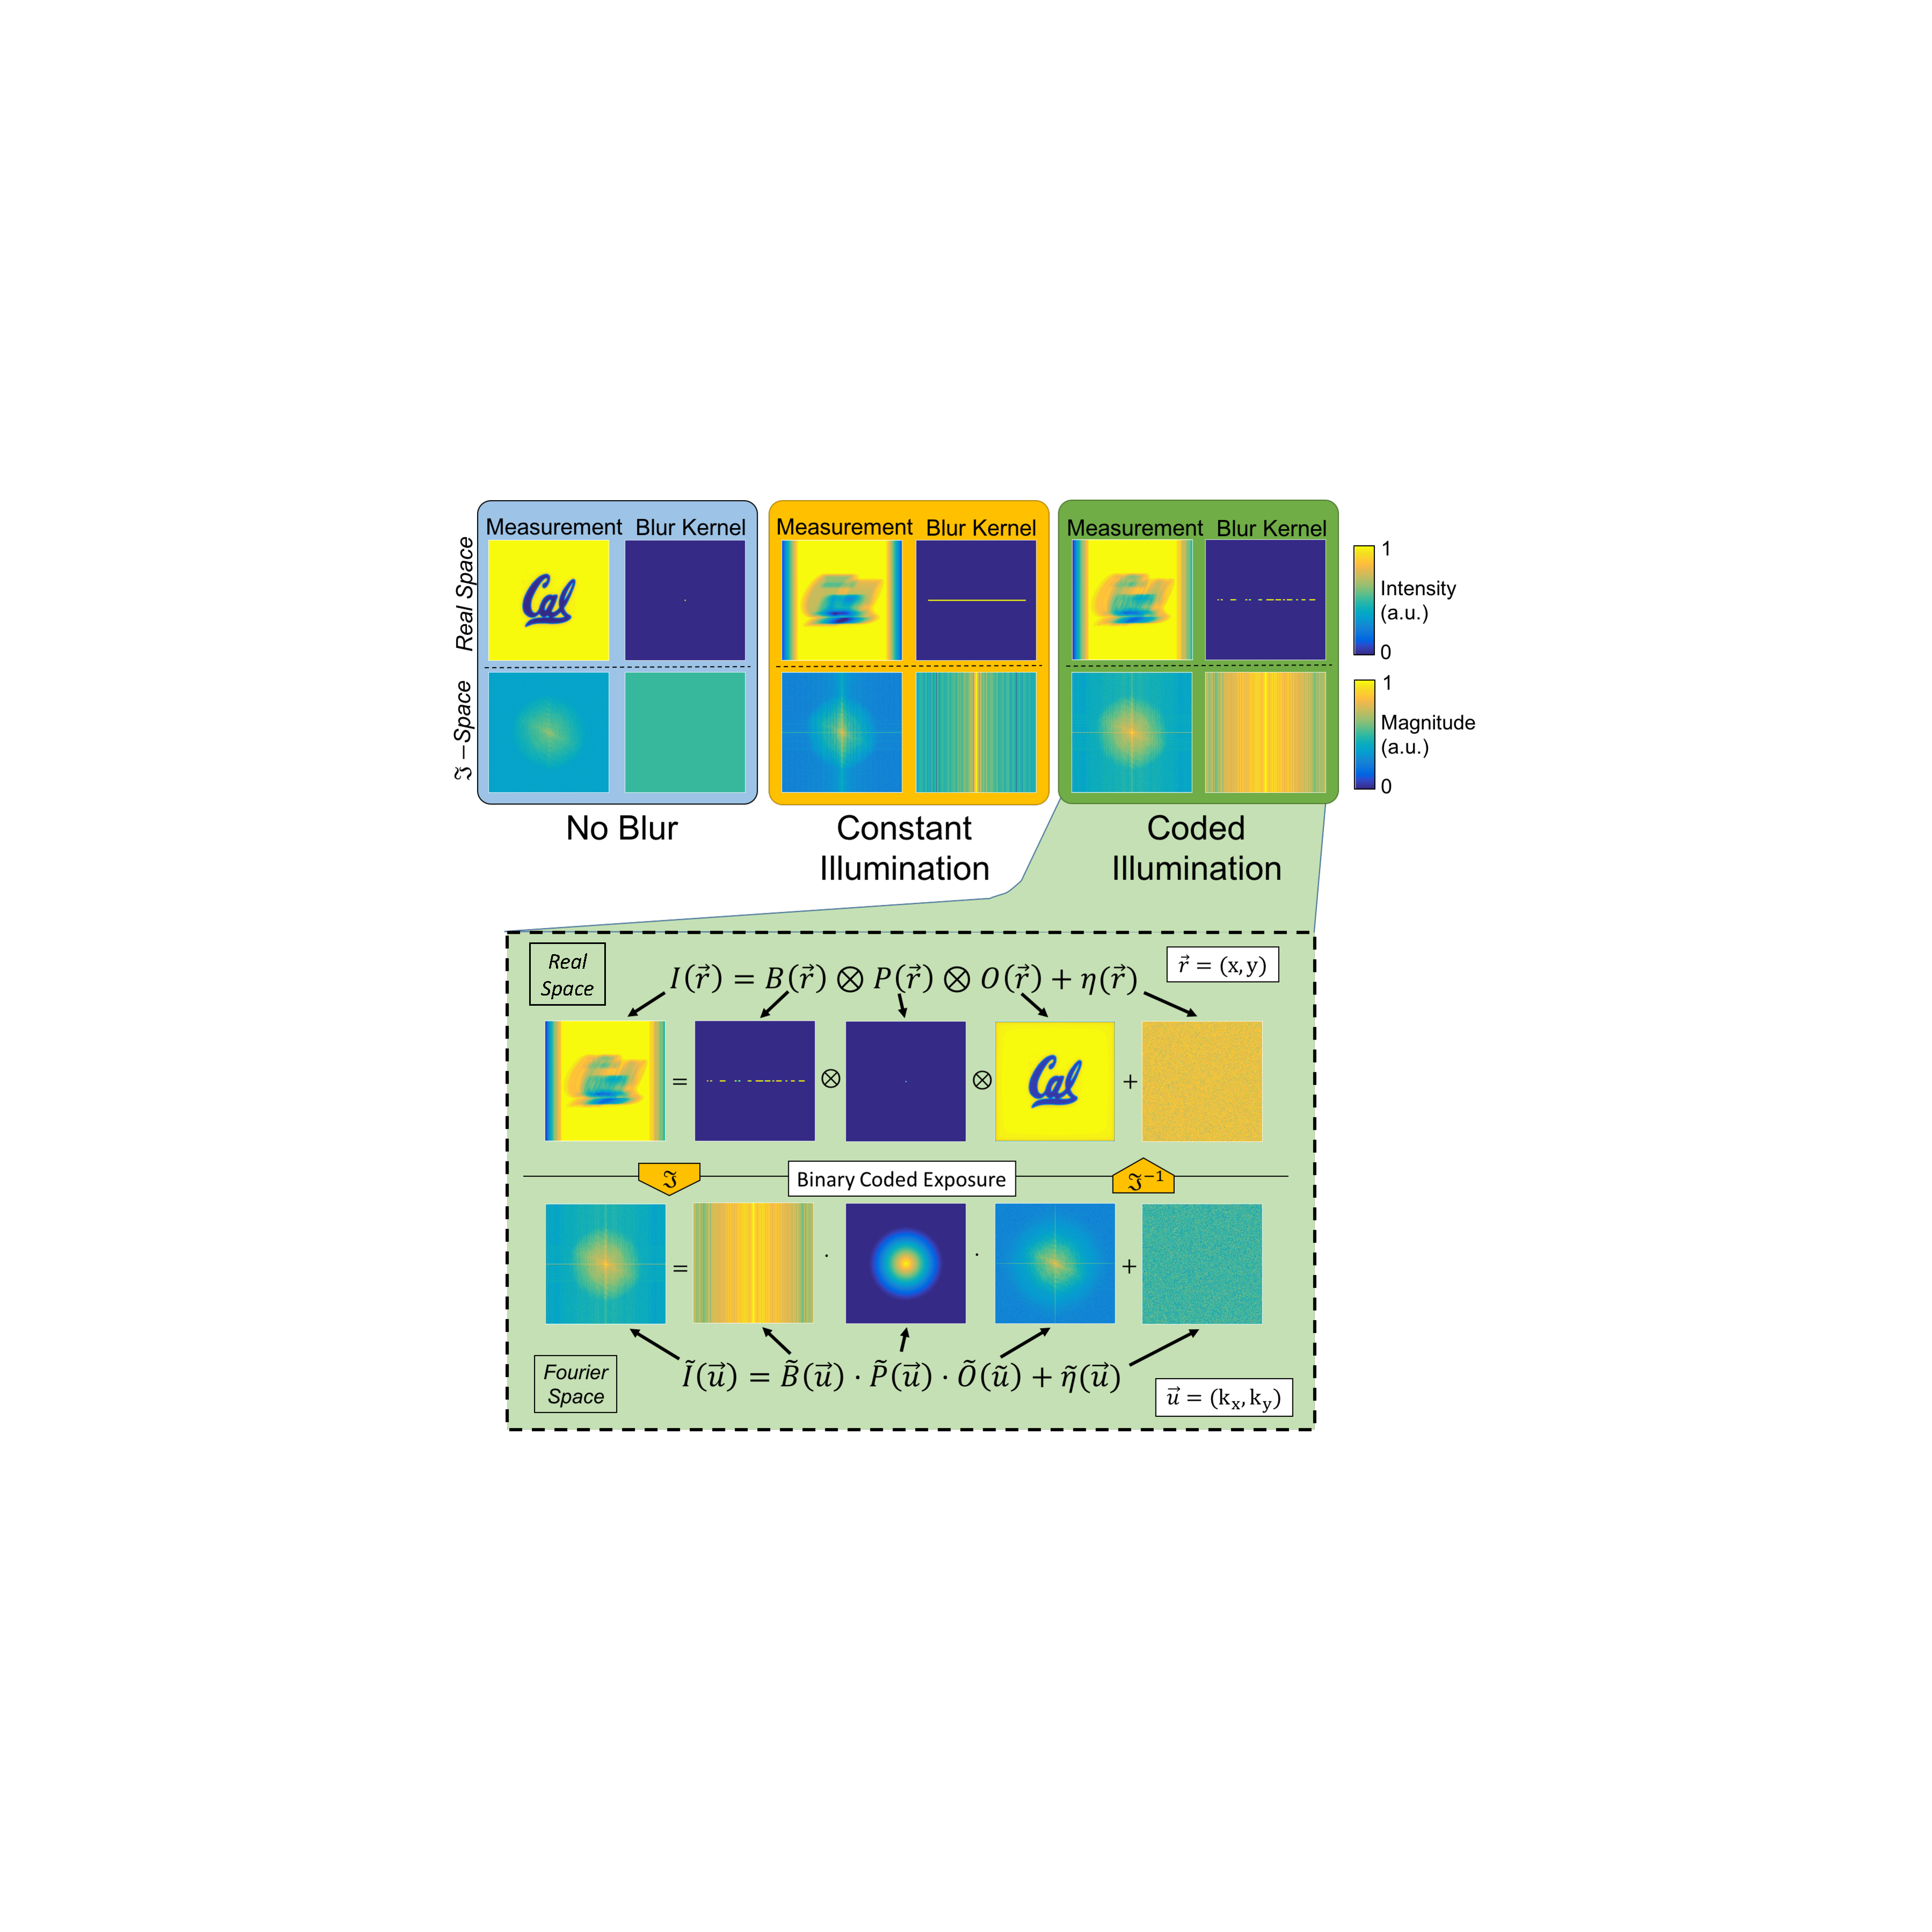
\includegraphics[width=1\textwidth]{deblur-fig1.pdf}
\caption{\label{fig:deblur}
Motion blur real-space and Fourier space representations. In the case of a static object, the object is filtered by the optical transfer function (OTF), assuming incoherent illumination. With motion blur, an additional convolution with a blurring function $B(\vec{r})$ causes attenuation in the frequency domain which acts as a cascaded linear filter on the object. In the case of coded blur, the transfer function is attenuated much less than in the conventional blur case. The colorbars are constant for real and fourier domain images respectively.}
\end{figure}

\section{Phase Imaging with Motion Deblur}
Phase Imaging using the Weak Object Transfer Function (WOTF) is highly compatible with motion deblur since both are modeled as linear convolutions on the same object. Chronologically, the results presented in Chapter 2 originated from the motion deblur problem, since we desired a method of recovering a blurred phase object from a single image. Recovering phase from multiple exposures is not considered in this chapter, but could be incorporated in future work. Our forward model in the frequency domain is a combination of the existing motion deblur model with the WOA. In the case of a single image, we model the blurred Intensity image as two separate convolutions, applied sequentially:

\begin{equation}
\tilde{I} = B * [ H_{\mu} * A + H_{\phi} * \phi]
\end{equation}

We can express the above equation as a block-wise matrix product in the Fourier domain, letting $\tilde{B}$, $\tilde{H}_{\mu}$, and $\tilde{H}_{\phi} $ be the diagonalized Fourier Transforms of the transform functions, and $\tilde{I}$, $\tilde{\mu}$, $\tilde{\phi}$ be the vectorized image and object components respectively:

\begin{equation}\label{forwardModelSingle}
\tilde{I} = \tilde{B} \cdot \begin{bmatrix} \tilde{H}_{\mu} & \tilde{H}_{\phi}\end{bmatrix}  \begin{bmatrix}\tilde{\mu}\\ \tilde{\phi} \end{bmatrix}
\end{equation}

The WOTF equations, which were defined in Chapter 2, are provided here again for a given illumination wavelength $\lambda $:

\begin{equation}\label{WOTFre_2}
\tilde{H}_{\mu}(\vec{f},\lambda) = \left[  P(\vec{f},\lambda) \star (P(\vec{f},\lambda)\cdot S(-\vec{f},\lambda))+ (P(\vec{f},\lambda) \cdot S(-\vec{f},\lambda)) \star P(\vec{f},\lambda)\right]
\end{equation}

\begin{equation}\label{WOTFim_2}
\tilde{H}_{\phi}(\vec{f},\lambda) = \frac{\lambda_0}{\lambda}\cdot\left[ P(\vec{f},\lambda) \star (P(\vec{f},\lambda)\cdot S(-\vec{f},\lambda))- (P(\vec{f},\lambda) \cdot S(-\vec{f},\lambda)) \star P(\vec{f},\lambda) \right],
\end{equation}

Combining measurements from the three color channels, we model the full over-determined system as:

\begin{equation}\label{forwardModel}
\begin{bmatrix}
\tilde{I}_{R}\cr \tilde{I}_{G}\cr \tilde{I}_{B}
\end{bmatrix}
= \begin{bmatrix}\tilde{B}_R & 0 & 0\cr 0 & \tilde{B}_G & 0 \cr 0 & 0 & \tilde{B}_B \end{bmatrix}
\times
\begin{bmatrix}\tilde{H}_{\mu,R} & \tilde{H}_{\phi,R}\cr \tilde{H}_{\mu,G} & \tilde{H}_{\phi,G}\cr \tilde{H}_{\mu,B} & \tilde{H}_{\phi,B}\end{bmatrix}
\times
 \begin{bmatrix}\tilde{\mu}\\ \tilde{\phi}\end{bmatrix}
\end{equation}.

As in \cite{raskar2006coded} and \cite{Ma:15}, we design our patterns such that the condition number of the blur kernel is minimized. By combining both motion deblurring and the linearized phase retrieval technique described in Chapter 2 (Eq. \ref{eq:Ha}, \ref{eq:Hp}), we can use knowledge of our WOTF as derived previously to influence our choice of $B$ to improve our overall phase and amplitude reconstruction from blurred data. The motion deblur problem as presented here will always degrade the result even with an ideal $B$ due to the constraints placed on the optimization problem. In the previous case, degradation due to the blurring operation was minimized by solving for a blur kernel with an optimally flat Fourier spectrum. This method, however, did not take into account the additional attenuation due to the OTF of the optical system.

\begin{figure}[h]
\centering
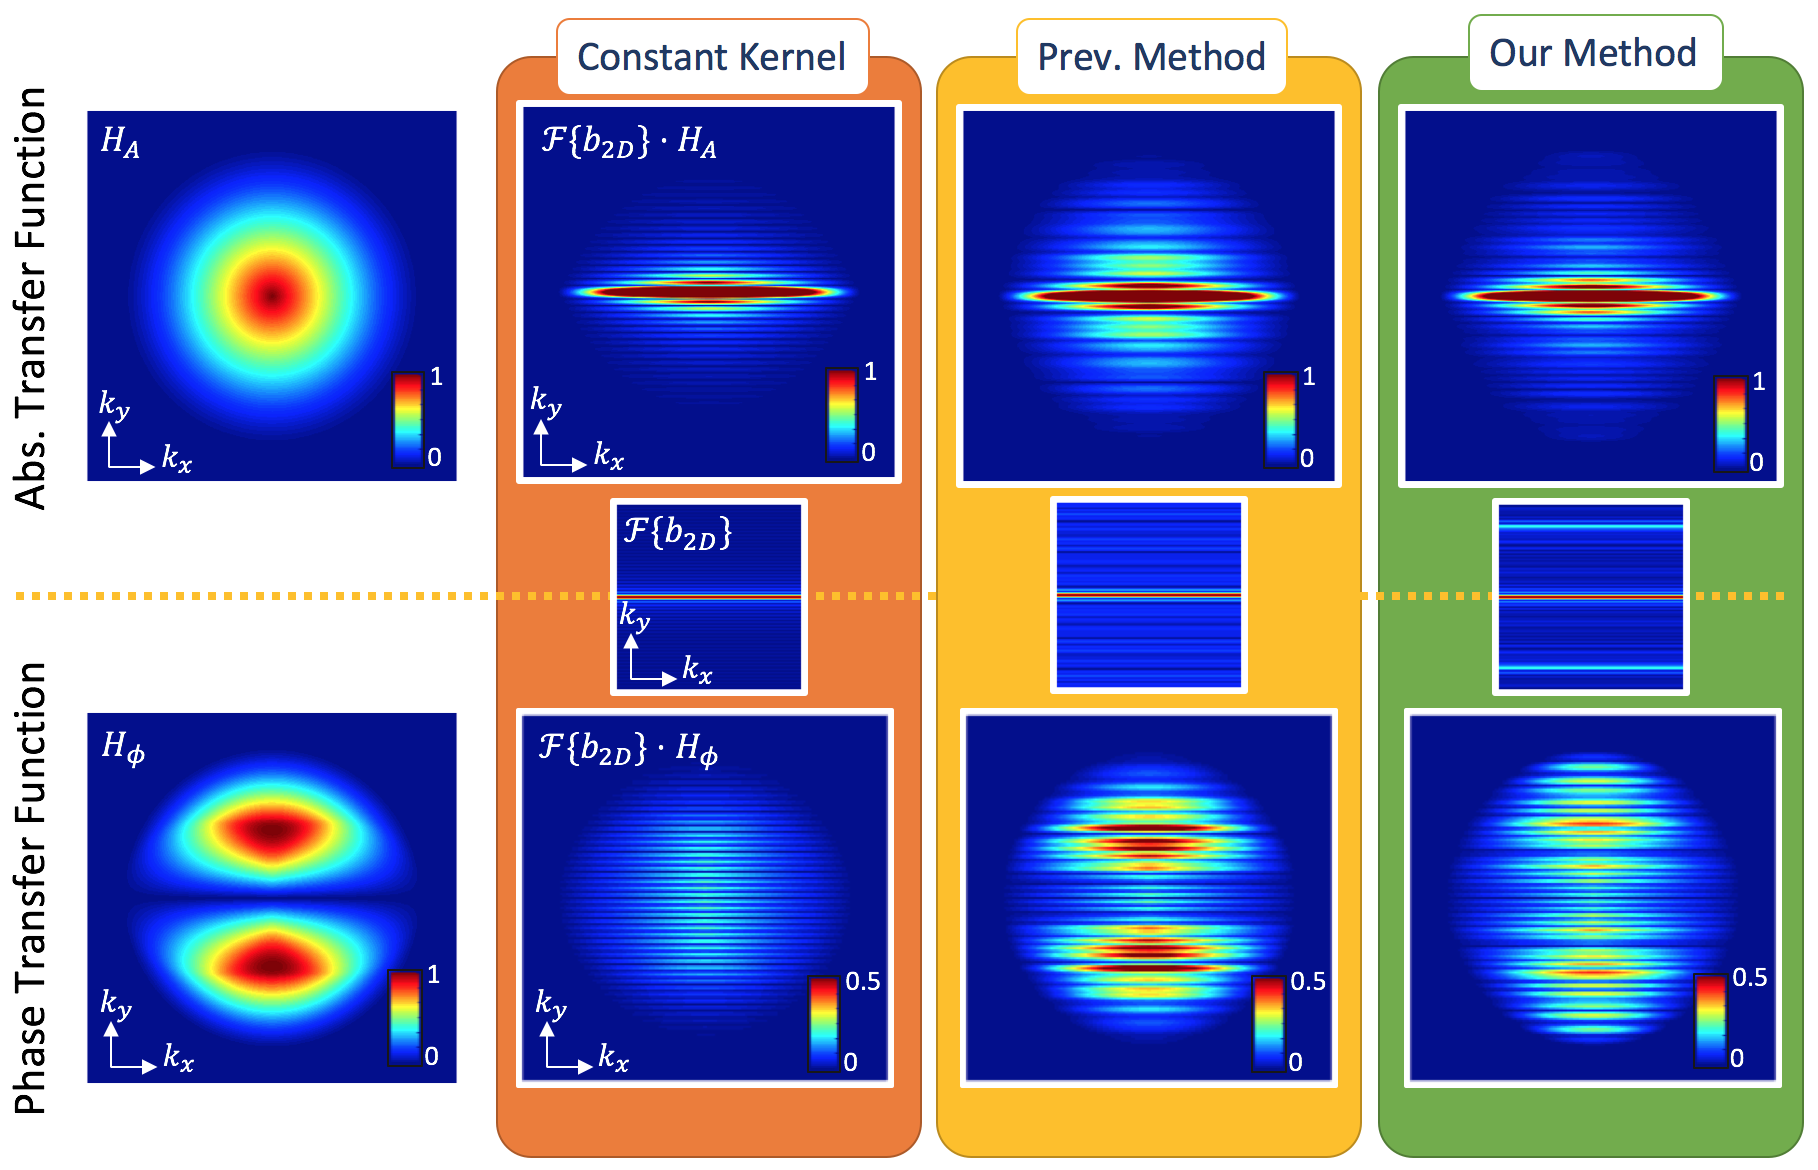
\includegraphics[width=1\textwidth]{deblur-fig2b.png}
\caption{\label{fig:deblurKernels}
Motion blurring kernels for 1D motion in the Fourier Domain.  \textbf{Left Column:} Unblurred absorption (top) and phase (bottom) transfer functions. \textbf{$2^{nd}$ Column}: Middle: Fourier transform of constant (non-coded) blur kernel. The top and bottom spectra in this column are the product of the unblurred transfer function and this center spectrum. \textbf{$3^{rd}$ Column}: Blurred transfer function spectra for temporal coding which does not consider WOTF structure. \textbf{$4^{th}$ Column}: Blurred transfer function spectra for temporal coding which emphasizes low and high frequencies based on WOTF structure.}
\end{figure}

Our improvement to the methods described in \cite{raskar2006coded} and \cite{Ma:15} is to consider the spectrums of cascaded filters in our system when designing our blur kernel. We can think of our sequential deconvolution problem as a single-step deconvolution which inverts the element-wise product of the blur kernel and WOTF's in the Fourier Domain. Therefore, the relative attenuation produced by the blur kernel at each frequency can be matched to reduce the degradation to highly attenuated frequencies in the WOTF, such as high frequencies in both amplitude and phase WOTF's, as well as low frequencies in the phase WOTF. The exact structure of this transfer function depends on the  pupil function of the optical system and design of the source. In practice, we note that the phase transfer function is of higher order than the amplitude transfer function (OTF), which generally means there are more zero crossings and values close to zero in the phase transfer function. Therefore, we will use the phase transfer function for optimizing the blur kernel.

To solve for the optimal blur kernel considering the WOTF, we modify Eq. \ref{eq:deblurKernelProb} to consider a 1D spectral reference $q$, which provides a measure of the attenuation imposed by the optical system at each spatial frequency in the blur kernel.

\begin{equation}
\begin{aligned}
& \underset{B}{\text{minimize}}
& & \frac{\max{|\tilde{B}\cdot \tilde{q}|}}{\min{|\tilde{B}\cdot \tilde{q}|}}\\
& \text{subject to}
& & \sum_{n=1}^N B[n] \geq \gamma N, \hspace{15pt} 0 \leq B[n] \leq 1 \hspace{5pt} \forall n
\end{aligned}
\end{equation}

For linear kernels, we chose $q$ to be the sum of the magnitude of the phase transfer function along the direction orthogonal to the blur direction as shown in Fig. \ref{fig:deblurKernels}. This quantity can be though of as a penalty function for attenuating each spatial frequency during the blurring process - if the OTF is already very low at a given frequency, the blur kernel should try not to attenuate this frequency significantly. Since the blurring filter is applied in hardware, this process improves noise performance for frequencies which are heavily attenuated by the optical system. It is important to note that this method will never improve resolution or noise performance beyond the static solution - however, it can greatly reduce the degradation due to the blurring process, making deblurring practical for high-speed quantitative imaging applications.

\begin{figure}[ph]
\centering
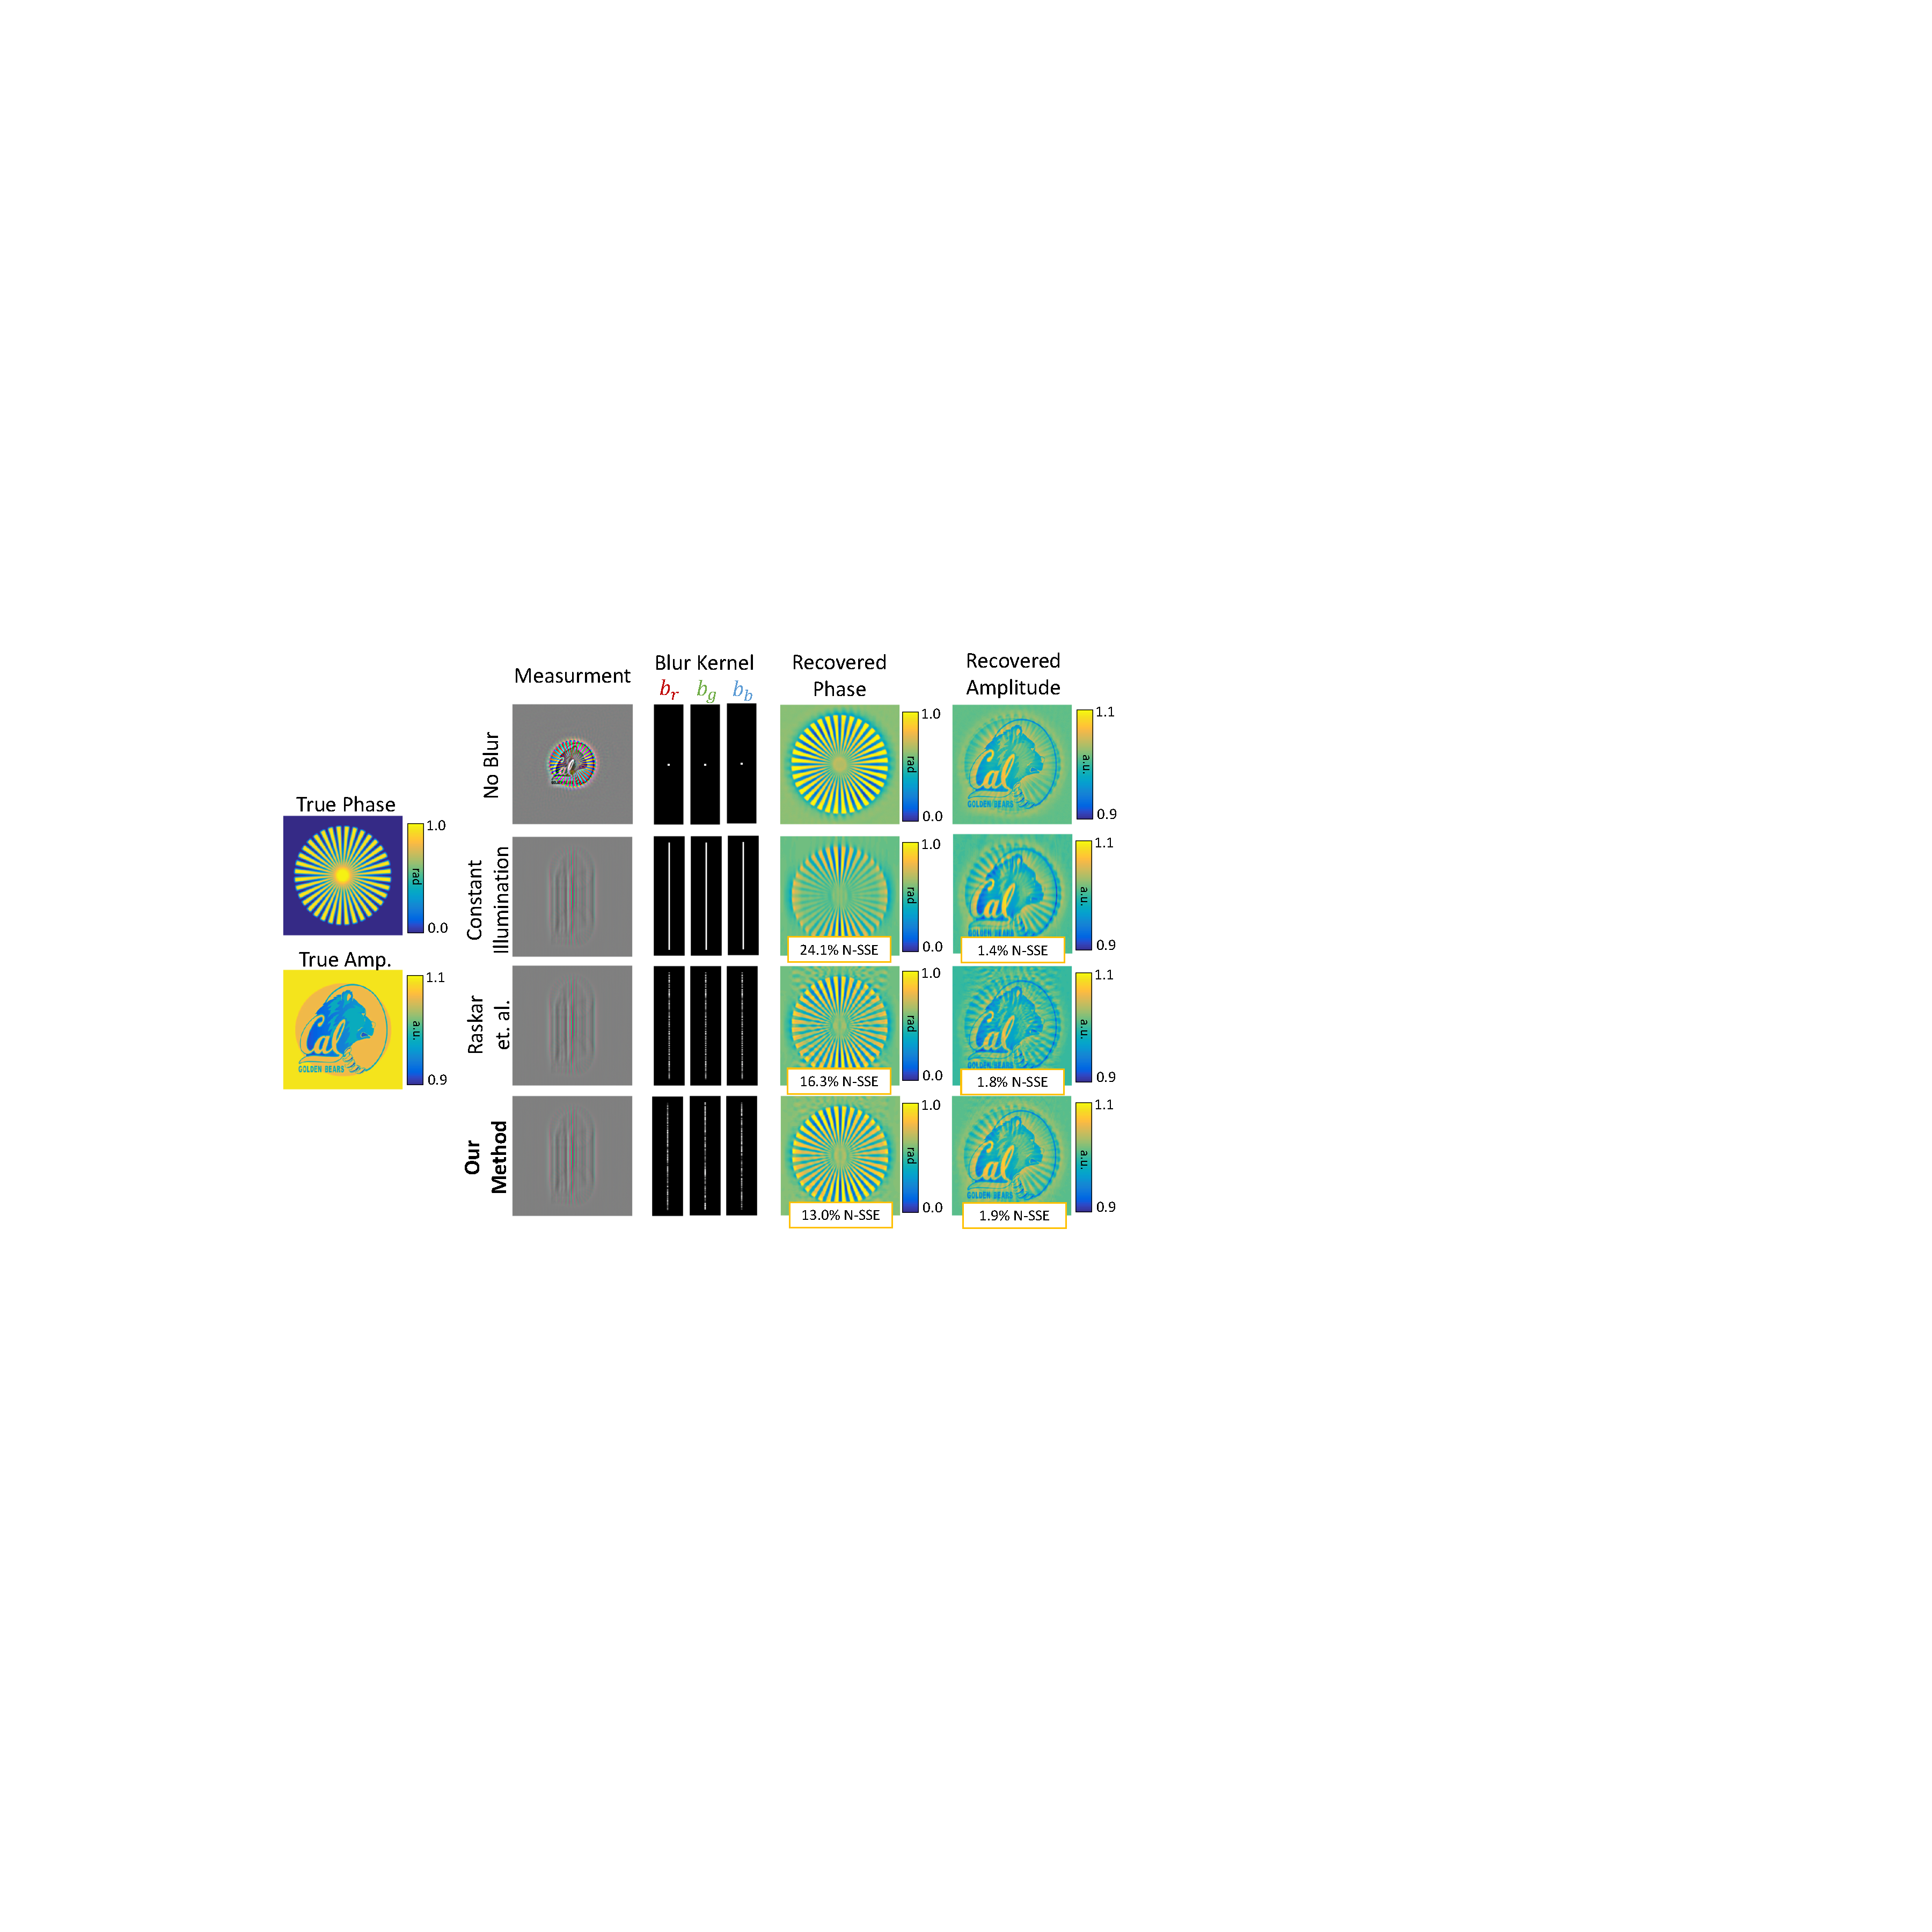
\includegraphics[width=0.9\textwidth]{deblur-fig3.pdf}
\caption{\label{fig:deblurSimulation}
Simulation results for phase retrieval from blurred images. \textbf{Top Row}: Phase and amplitude retrieval of a stationary sample. This serves as our best-case reconstruction for the blurred images. \textbf{Second Row}: Phase and amplitude retrieval of a blurred sample using constant illumination. This is the degenerate solution. \textbf{Third Row}: Deblur using a coded blur kernel as in the previous methods. The result improves significantly over the constant illumination case, but is still missing features in phase. \textbf{Fourth Row}: Deblur using our coded kernels}
\end{figure}

\section{Validation}
\subsection{Simulation}
Simulation results are shown in Fig. \ref{fig:deblurSimulation}. Here we show a static sample, deblurring without coded illumination, deblurring with the previous method (no spectral reference), and deblurring using our method, which accounts for the optical system transfer function. In this simulation we note that the normalized sum-squared error (N-SSE) in phase is reduced significantly in our method. The amplitude N-SSE did increase slightly using our method, which is likely due to the fact that we used the phase WOTF for generating our blur kernels instead of amplitude. The choice of which WOTF to use could be application-dependent.

\subsection{Experimental Results}

Our system consists of a commercial Nikon AZ100 microscope using a 1$\times$ 0.10 NA objective, a Bayer-patterned SCMOS camera (PCO.edge 5.5), an XY stage with linear encoders, (Prior H117), and illumination from 23 multi-channel LEDs (Jameco 2128500) arranged in a hexagonal pattern using a laser-cut holder for positioning. The LEDs were placed approximately 160mm from the sample to match the spacing such that the outer LEDs illuminate the sample from angles just inside of the NA of the microscope. This is done to ensure maximum phase contrast and bandwidth (resolution) of the system. The LEDs are controlled using a Teensy 3.2 microcontroller, which can be dynamically programmed. Camera exposures, stage movement, and illumination modulation are controlled using open-looped feedback with 5ms synchronization resolution, limited by the update speed of the LED array. This system is shown in Fig. \ref{fig:deblurSystem}.

\begin{figure}[ph]
\centering
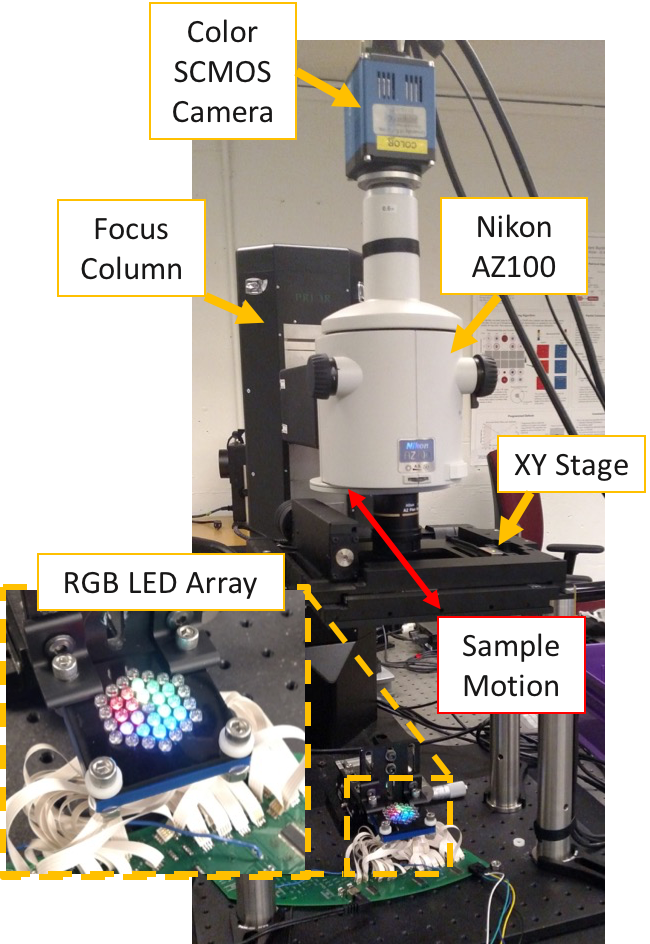
\includegraphics[width=0.8\textwidth]{deblur-fig5.png}
\caption{\label{fig:deblurSystem}
Experimental setup for motion deblurring. The tri-color LED array provides fast illumination coding in time, angle, and color. The LED array can be programmed dynamically using a Teensy micro-controller and has a maximum update speed of approximately 250 Hz. The LED array is synchronized with the linear motion stage and camera in hardware to provide precise system synchronization.}
\end{figure}

Our forward model considers the case where our LED illumination is incoherent and discrete, both spatially and temporally. We assume each emitter has three coincident emitters for Red ($\bar{\lambda} = 625$), Green ($\bar{\lambda} = 525$), and Blue ($\bar{\lambda} = 470$), wavelengths, which propagate through the optical system independently of each other and are detected separately by the bayer filter of our color camera. We assume a sample which is non-dispersive and unstained. A velocity of 25mm per second was used for sample movement, but this could be increased by improving hardware synchronization. Blur kernels were calculated using the calibrated phase WOTFs for each color channel separately, considering the spacing of k-space due to wavelength.

Experimental reconstructions are shown in Fig. \ref{fig:deblurResults}. To test our method, we used a micro-lens array (Fresnel-Tech 605) as our sample due to it's well-defined geometry. Fig. \ref{fig:deblurResults} shows reconstructions for the static case, previous method, and our method. While the sample amplitude is relatively unchanged, the phase reconstructions clearly show that accounting for the spectral reference provides better results than optimizing the blur kernel alone. This supports our claim that image degradation from blurring can be reduced significantly, but not eliminated, using our method.

\begin{figure}[ph]
\centering
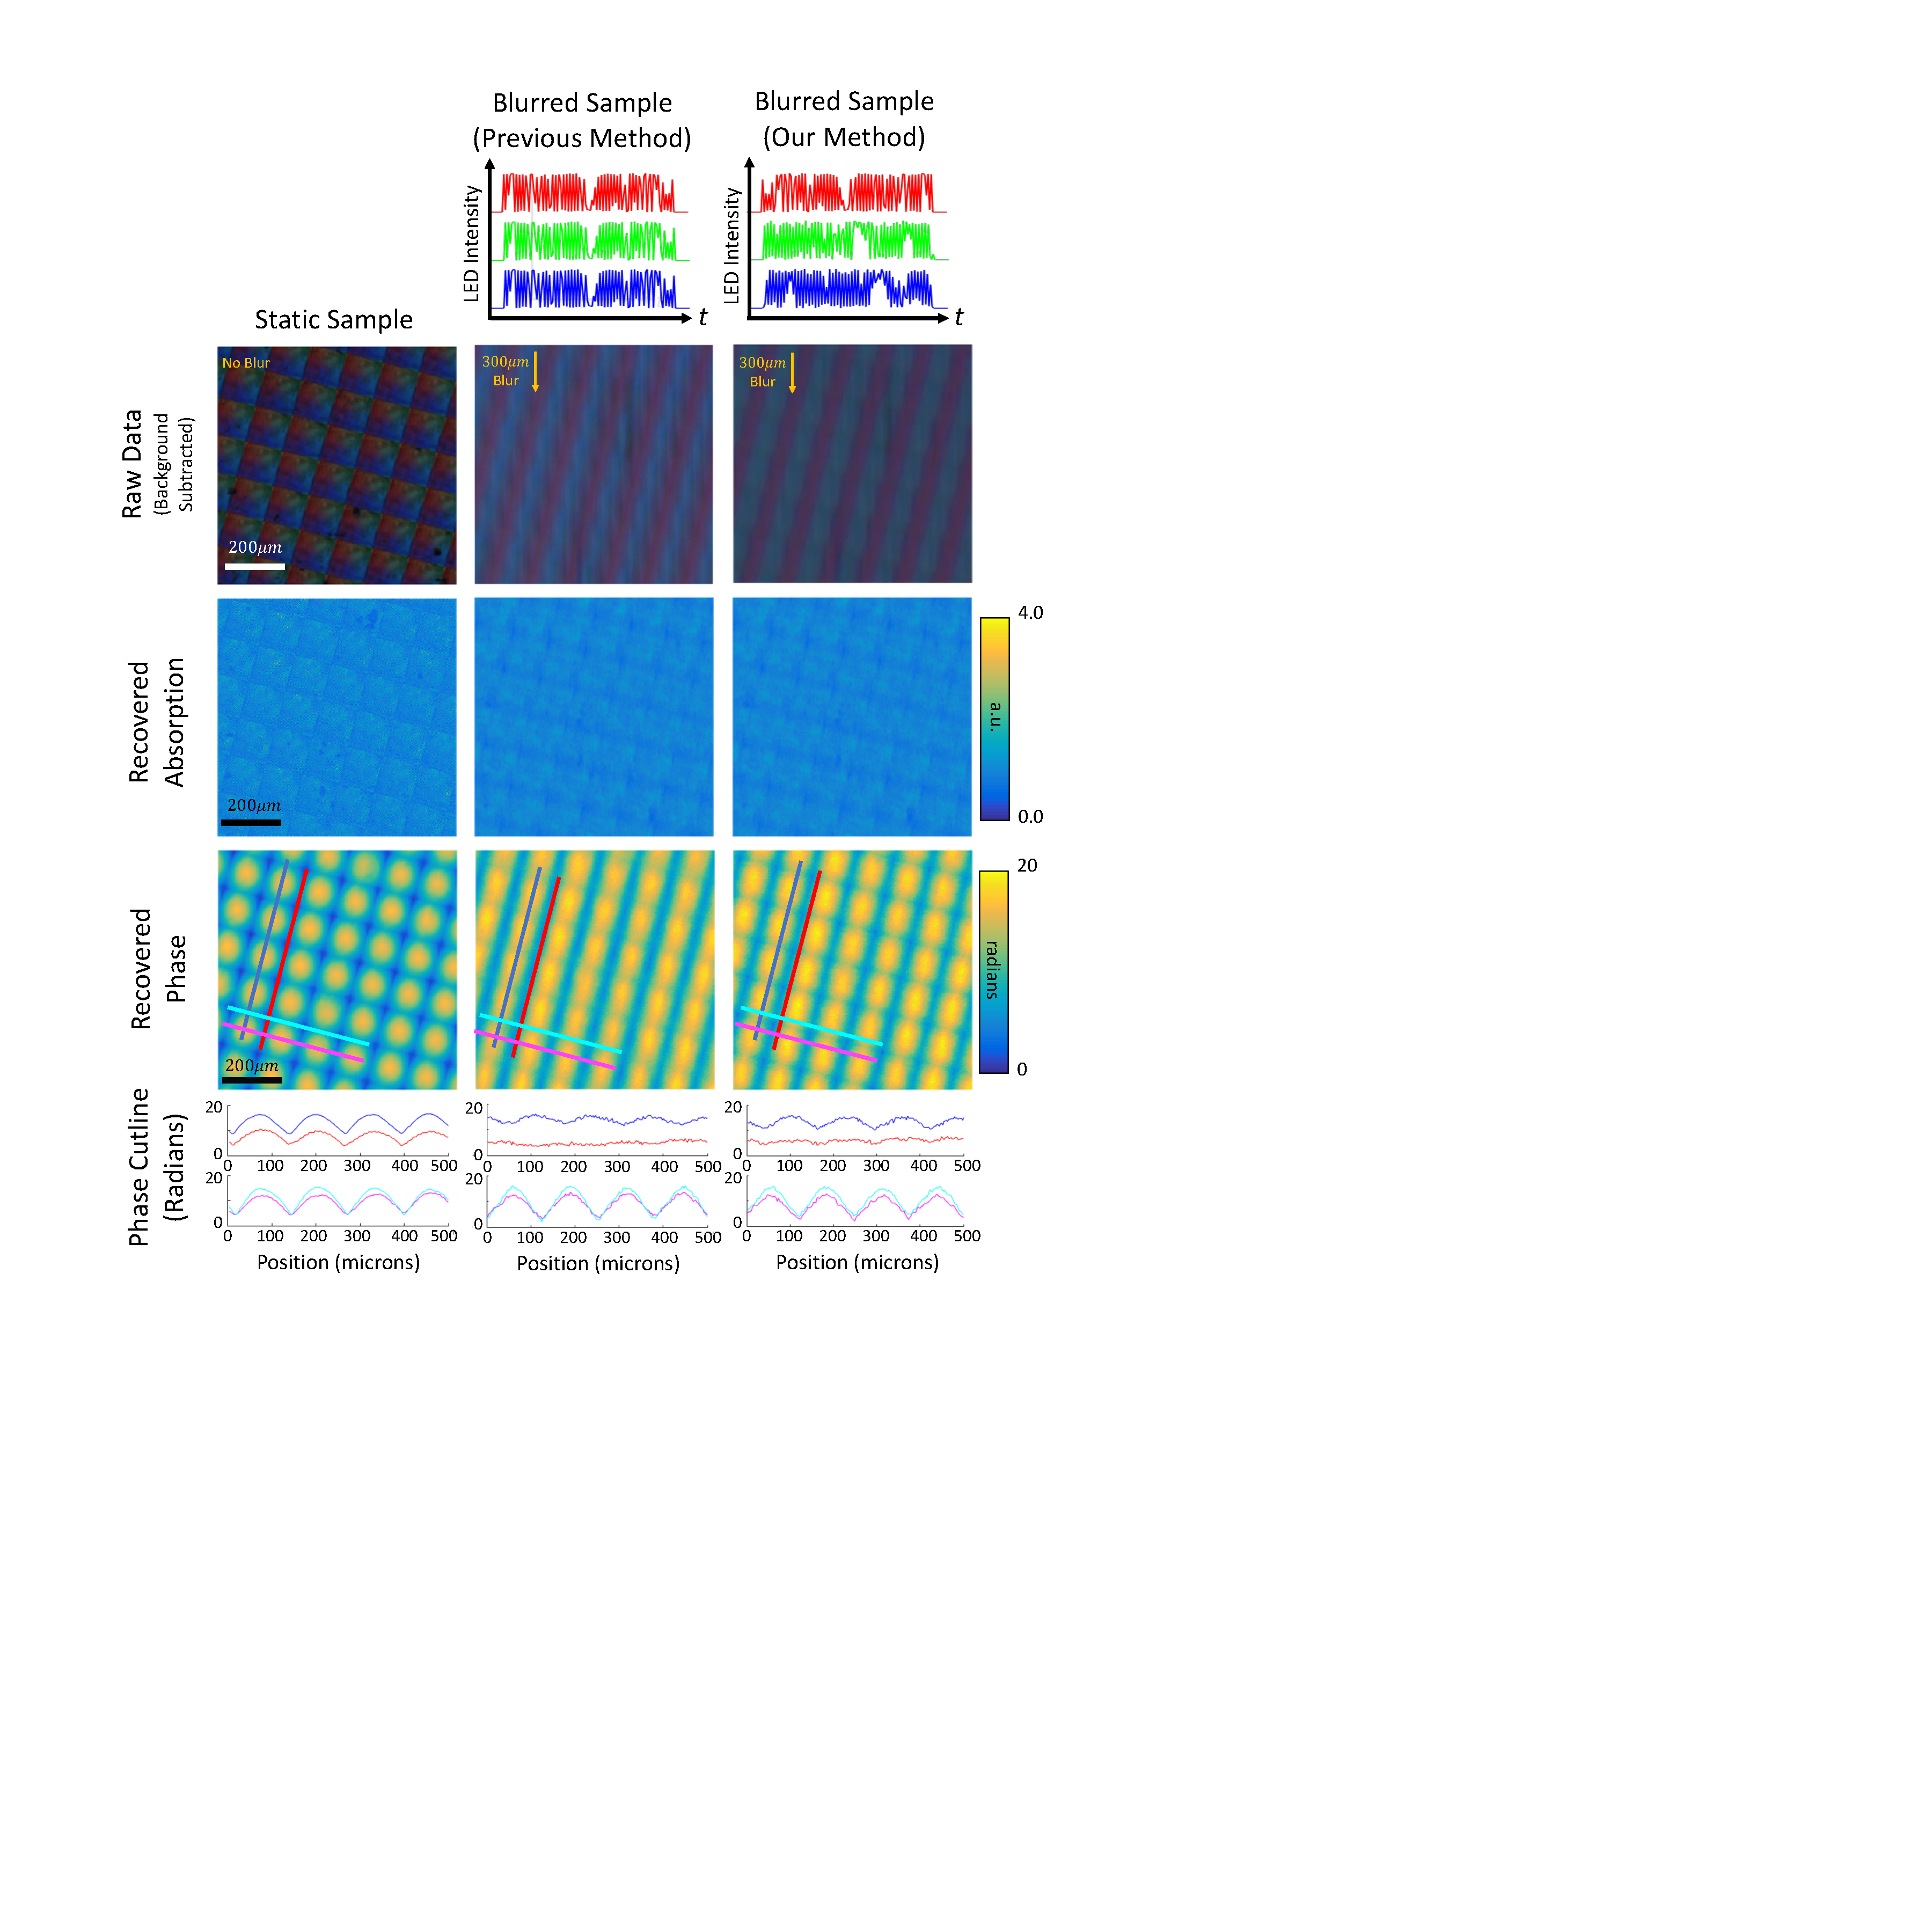
\includegraphics[width=0.8\textwidth]{deblur-fig4.pdf}
\caption{\label{fig:deblurResults}
Experimental results for motion deblur of a moving sample (Fresnel Technologies 605 micro-lens array).}
\end{figure}

\chapter{A Smartphone-Based Portable Computational Imaging System}
\section{Portable Microscopy}
Optical microscopy is an important tool for disease screening and diagnosis throughout the world. Significant resources have been devoted to developing portable and affordable compact microscopes for remote clinical applications~\cite{Zhu2011, switz2014low, smith2011cell, maamari2013mobile,C4LC00010B,Vashist2014,steenblik2005lenses,10.1371/journal.pone.0098781,boppart2014point,Greenbaum17122014,mudanyali2010compact,tseng2010lensfree}. Compact microscopes based on mobile phones, including CellScope~\cite{10.1371/journal.pone.0006320,10.1371/journal.pone.0096906}, have demonstrated that microscopy can be effectively performed outside of hospitals and diagnostic laboratories by minimally trained healthcare workers, that images can be transmitted for confirmation of diagnosis, and that phone-based computational analysis can be used to provide automated diagnosis. These mobile microscopes complement a host of other new devices for health monitoring on smart phones~\cite{oncescu2014cholesterol, pamplona2010netra, eyeexaminer, peekvision}. 

\section{Computational CellScope}
Here, a new variation of the CellScope microscope is demonstrated which incorporates recently developed techniques of computational illumination~\cite{Zheng2011, Tian14, zijiMulti} to enable new imaging modalities, including darkfield, phase imaging and digital refocusing. Using the same LED array illumination, Computational CellScope also implements lightfield digital refocusing, so that a sample focus can be changed after the fact (without mechanically changing focus) and 3D image stacks can be extracted for both intensity and phase modes. Further, constant focus correction (auto-focusing) can be implemented in post-processing for long time-lapse studies. The digital refocusing is achieved by sequentially illuminating the sample from each of the LEDs that lie inside the numerical aperture (NA) of the objective, then post-processing to form a stack of through-focus images of intensity~\cite{Ng2005,Zheng2011} or phase contrast~\cite{Tian14}. For thick samples, the result also provides a 3D reconstruction of the sample, similar to limited angle tomography.

The computational illumination techniques used here have been previously demonstrated in a traditional microscope using a planar LED array ~\cite{Zheng2011,Zheng2013,Tian14,zijiMulti,tian20153d}. The purpose of the LED array is to flexibly pattern illumination angles at the sample by turning on different sets of LEDs corresponding to different illumination angles. The optimal arrangement of LEDs, however, is not planar but rather a dome shape ~\cite{Dominguez:14}, which we utilize here. The domed arrangement provides significant improvements in intensity uniformity and light throughput, since LEDs can be directionally biased and arranged at uniform radius from the sample. These benefits contribute to increased signal-to-noise ratio (SNR) in the darkfield images, allowing effective high angle illumination patterning and shorter exposure times. 

The flexibility and speed of the programmable LED array illuminator, as well as the lack of moving parts and low cost, make the hardware very amenable to modification as a CellScope attachment. In order for our device to be practically useful in the field, we have here enforced the requirement that all of our processing and control be performed on the smartphone, without use of a PC. Thus, the device can be field-deployable as a simple add-on to CellScope. In the following sections we detail the design and performance of the hardware and software of our new Computational CellScope device.

\begin{figure} [h]
\begin{center}
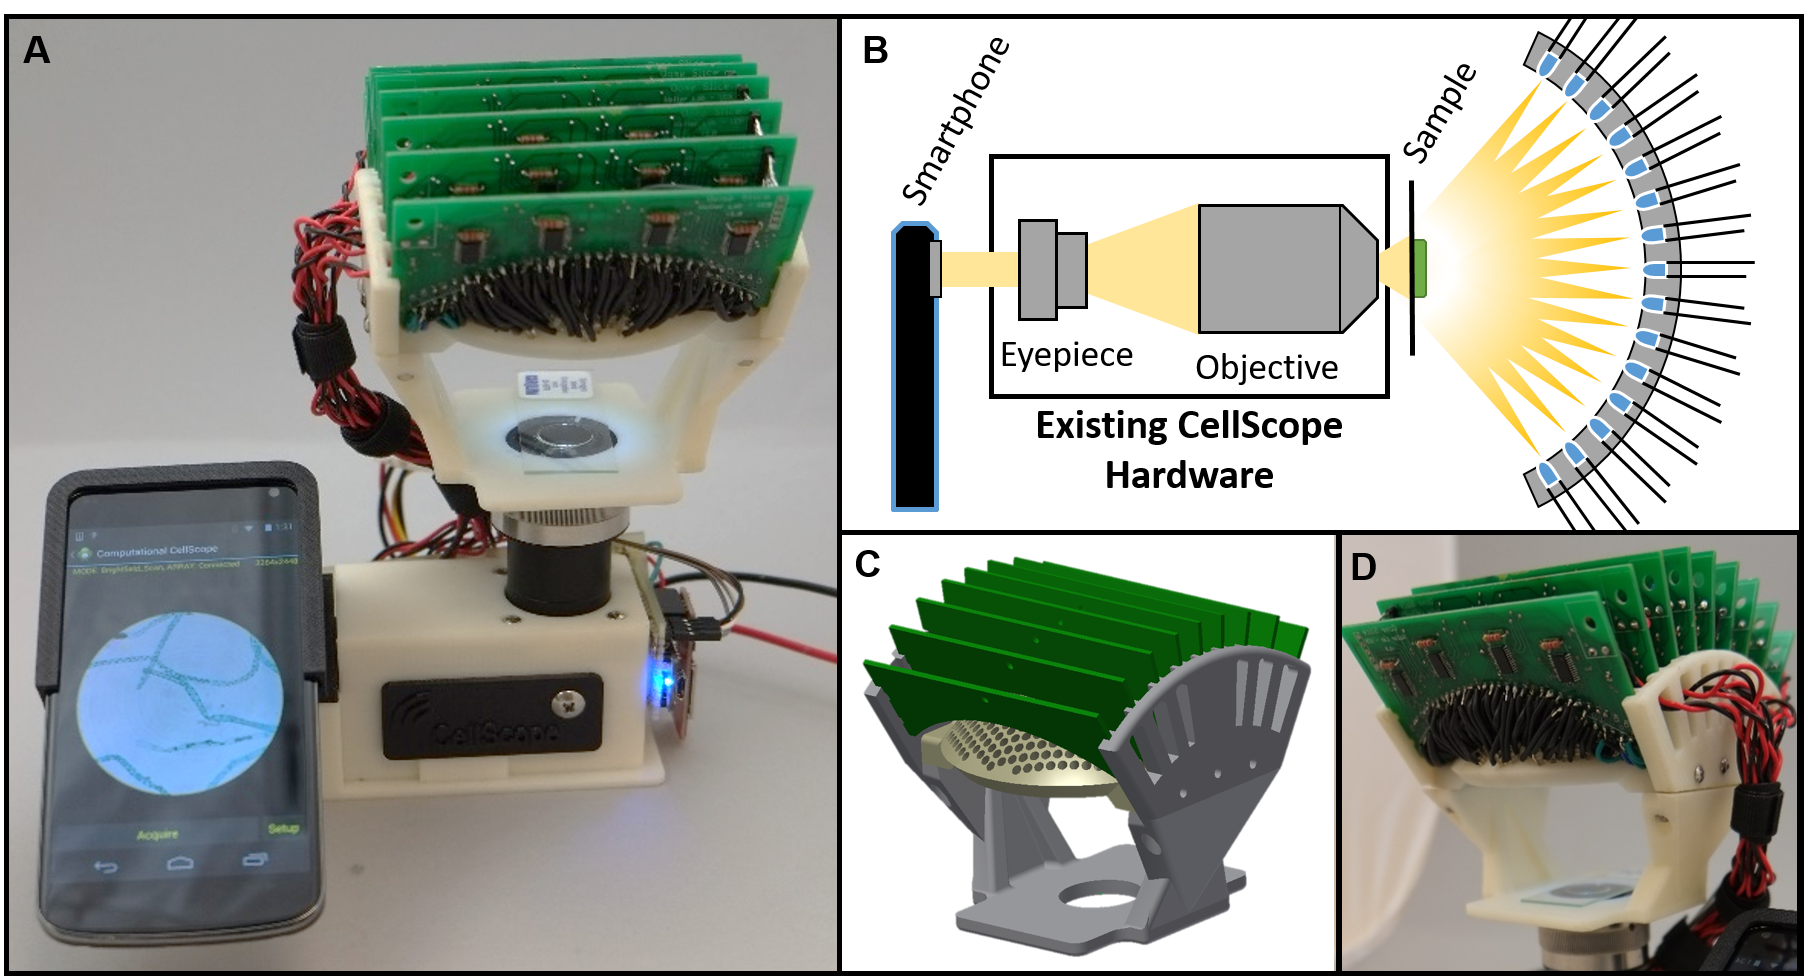
\includegraphics[width=\textwidth]{ccs-fig1.png}
\end{center}
\caption {{Computational CellScope.} {a).} Device observing a sample using a Nexus 4 smartphone. {b).} Optical schematic of the CellScope device with our custom-made domed LED illuminator. {c).} CAD assembly of the dome. {d).} Assembled dome and control circuitry.} 
\label{fig:device} 
\end{figure}

\section{Domed LED Illumination}
The Computational CellScope hardware involves a custom-built domed LED illuminator attached to an inverted variant of the CellScope smartphone-based microscope platform (see Fig. 1). The CellScope used here is a finite-conjugate transmission microscope coupled to an Android-based Nexus 5 smartphone (LG Electronics/Google) as described in in Skandarajah, et al.~\cite{10.1371/journal.pone.0096906}. Our domed illuminator hardware is compatible with all smartphones and tablets that are used with the existing CellScope, including the iPhone 4S, 5, 5S, and 6 (Apple, Inc.), as well as several Android devices. Phones are mounted via modular 3D printed mounts adapted to each specific smartphone model. Hardware changes were entirely on the illumination side, where we have replaced the original single LED light with our domed illuminator consisting of 508 individually addressable broad spectrum (white) LEDs. Our domed LED arrangement was inspired by the opto-mechanical geometry of the AWARE gigapixel camera~\cite{brady2012multiscale}. LEDs are uniformly distributed in an (approximately) hexagonal packing pattern across a 77 degree cone of angles corresponding to an illumination NA of 0.62. Thus, darkfield imaging is feasible for objectives with NA smaller than 0.62 (as illustrated in Fig.~\ref{fig:dome}f), and both phase and digital refocusing are possible for all objective NAs. The dome assembly was is secured to a custom stage that attached to the top of the CellScope objective; the stage and circuit board holders were 3D printed using low-cost ABS plastic. In general, the design is modular and features simple electronics, including the use of the inexpensive and widely used Arduino micro-controller platform. Phone mounts can be swapped out for upgrading to new models and objectives can be replaced for varying the magnification of the system. While our addition involves custom LED drive circuitry and a 3D printed structure, complexity was kept low to preserve the low-cost nature of CellScope. Part counts, cost and especially size may be further reduced in design-for-manufacture. The size of the illuminator could be reduced to essentially the dimensions of the dome itself, and cost could be comparable to the price of a modern smartphone, matching and improving upon the functionality of a full-size microscope at a fraction of the cost.  

% Dome design figure
\begin{figure} [h]
\begin{center}
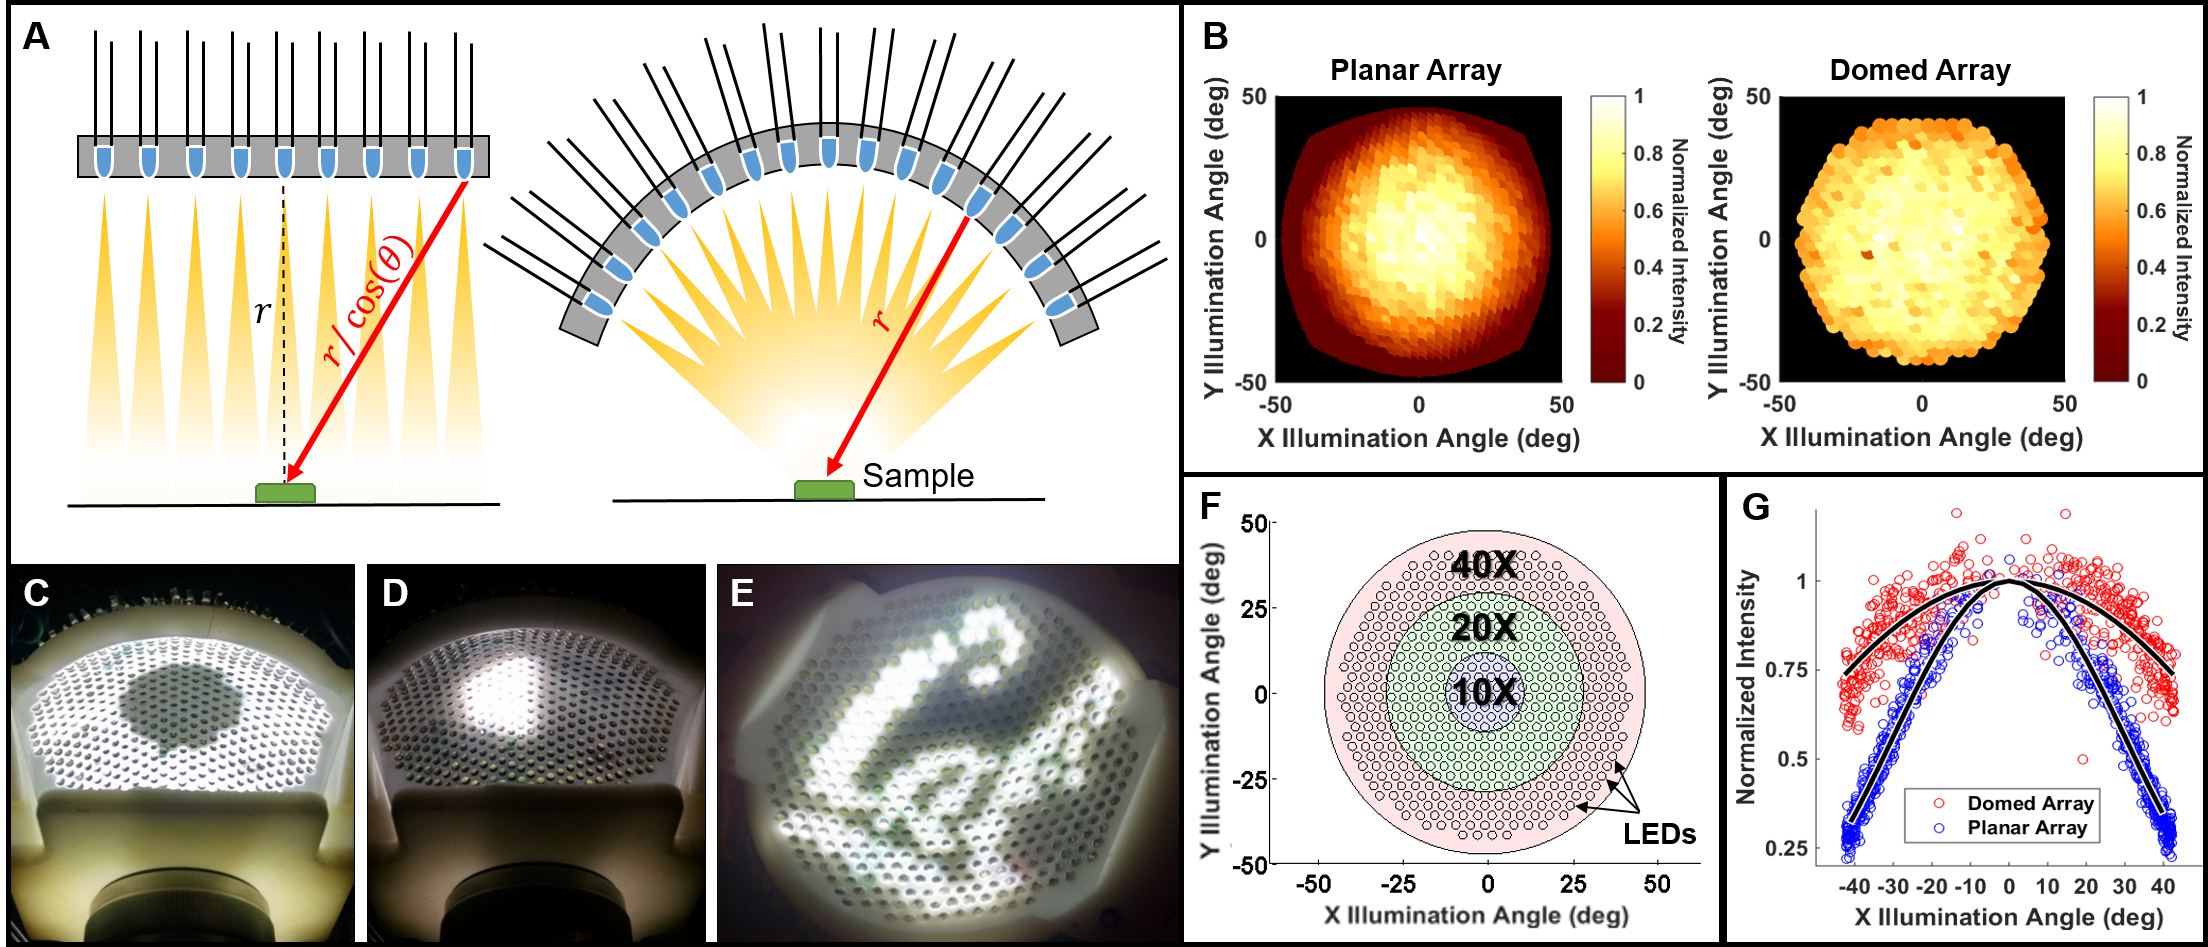
\includegraphics[width=\textwidth]{ccs-fig2.png}
\end{center}
\caption {{ Domed LED Illuminator.}{a)} Illumination pattern used to acquire dark field images with a 0.25 NA objective.
{b)} Illumination pattern used to synthesize differential phase contrast images with a 0.25 NA objective.
{c)} Illustration of the arbitrary illumination patterning capabilities of the device.
{d)} Normalized mean pixel intensities measured at the sensor for the planar and domed arrays. Intensity decreases as a function of angle in both cases, but much more strongly in the case of the planar geometry. Values were normalized to the central LED's brightness in both cases.
{e)} Visual comparison of a planar LED array with a domed array. Since the intensity of a spherical wave drops as a function of the inverse square of radius, the illumination at the sample depends on the distance between the LEDs and the sample. In the planar case (left), LED distance $r$ increases as a function of illumination angle, causing weaker illumination at higher angles. A domed LED array (right) eliminates this variation ($r$ is constant). 
{f)} Plot illustrating the relative objective NA for several common magnifications, as compared to our dome's LED placement (small black circles).
{g)} Normalized measured intensity falloff as a function of angle relative to the optical axis for the domed and planar LED arrays. Falloff is proportional to $\cos{\theta}$ for the domed geometry and $\sim\cos^4{\theta}$ for the planar geometry. Black lines are $\cos{\theta}$ and $\cos^4{\theta}$ fits for the domed and planar geometries, respectively. The domed geometry exhibits significant improvements in intensity at large angles of illumination. 
}
\label{fig:dome} 
\end{figure} 

The domed LED arrangement provides significantly better light efficiency than the planar LED arrays used in previous work, enabling shorter acquisition times and more efficient power use. These advantages could be crucial for mobile microscopy applications where power is a scarce resource, and shorter exposure times reduce motion blur artifacts due to unstable experimental conditions. The power benefits are a result of two phenomena, shown in Fig. ~\ref{fig:dome}e. The first is that off-axis LEDs in a planar array will have a larger LED-to-sample distance and thus decreased intensity at the sample. For example, if we assume that each LED is a point emitter, the intensity falloff due to increased distance can be expressed as $I(\theta) = I_0 \cos^2{\theta}$, where $I_0$ is the intensity at the sample from the on-axis LED and $θ$ is illumination angle. The second improvement in light efficiency comes from the fact that LEDs have significant angular variation in intensity (typically emitting more light in the forward direction). In a planar array, the LEDs at higher angles provide less effective illumination, a problem corrected by the dome geometry, where all LEDs are radially oriented. In both the domed and planar geometries we note that intensity further decreases with a final factor of $\cos{\theta}$ due to the smaller profile of objective window when viewed off-axis; combining these factors and assuming a Lambertian ($\sim\cos{\theta}$) angular dependence for physical (non-point-source) LEDs results in an expected intensity falloff of $\sim\cos^4{\theta}$ for the planar geometry but only $\sim\cos{\theta}$ for the domed geometry, a vast improvement at high incidence angles. Thus, the difference between geometries is proportional to $cos^3{\theta}$, or a factor of $> 50\%$ at $40\degree$ and $99\%$ at $77\degree$ incidence, having a substantial impact on required exposure times. Such behavior matches well with our experimental measurements (Figs.~\ref{fig:dome}d,g), where the measured intensity is shown for both geometries out to 40˚ incidence. Variations in intensity between LEDs may also come from electrical variations such as batch differences in controller chips and resistor tolerances.

% Contrast method comparison figure
\begin{figure}
\begin{center}
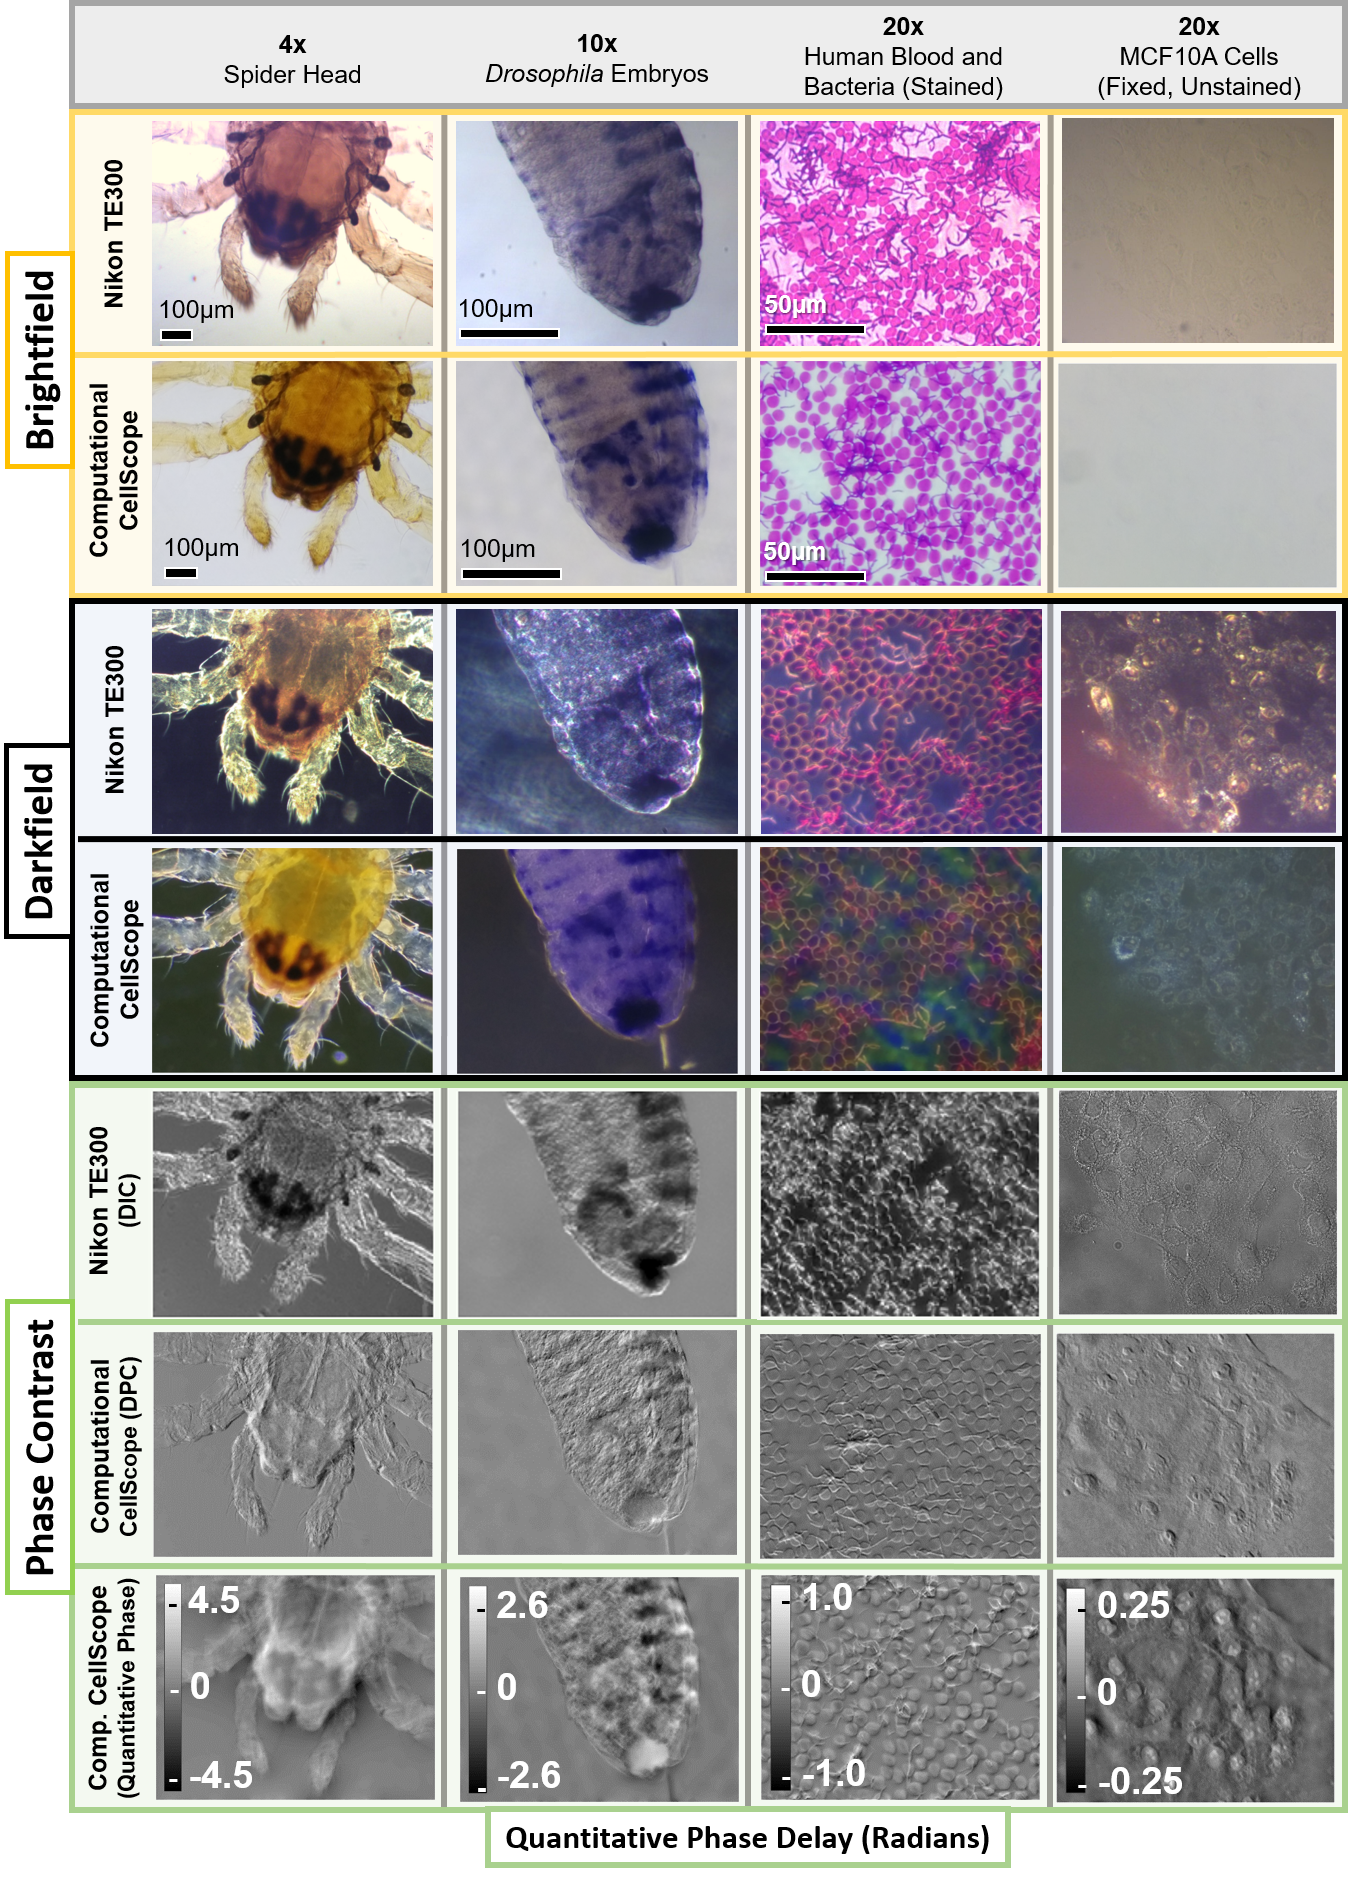
\includegraphics[width=0.67\textwidth]{ccs-fig4.png}
\end{center}
\caption {{Image Results Compared to a Standard Microscope.} Computational CellScope acquires brightfield and darkfield images of similar quality to a standard upright microscope (Nikon TE300) without the use of hardware inserts. Additionally, it enables phase imaging using Differential Phase Contrast (DPC), which contains similar information to standard phase contrast imaging, and can be inverted to obtain quantitative phase of the sample (bottom row). Differences in color shades are caused by the relative differences in hue of the halogen lamp and the white LEDs. Note the additional dark features in DIC results, as compared to DPC, illustrating mixing of phase and absorption information in DIC. In the rightmost column, we show images for an unstained transparent sample, illustrating the utility of phase imaging methods for label-free imaging.
}
\label{fig:contrastcomparison}
\end{figure} 


\section{Multi-Contrast Imaging}

To achieve brightfield, darkfield and phase contrast simultaneously, we time-multiplex images taken with different LED patterns and post-process them on the smartphone to synthesize pseudo-real-time multi-contrast imaging, as in~\cite{zijiMulti}. Brightfield images correspond to illumination by LEDs that lie within the cone of angles described by the objective numerical aperture (NA). Darkfield images are obtained by illuminating the sample from angles beyond the angular acceptance of the objective (Fig.~\ref{fig:dome}a)~\cite{Zheng2011}. Since different objectives have different NA, one must specify in the software which objective is being used, with larger NA corresponding to a larger brightfield region of LEDs. Our dome is designed to enable darkfield contrast for any objective of NA$<0.62$, roughly corresponding to a typical 40$\times$ objective.

Phase contrast can be achieved in a single-shot image by any asymmetric illumination pattern~\cite{kachar1985asymmetric,Dodt01101999}. Here, we choose to employ a differential phase contrast (DPC) scheme~\cite{Hamilton1984a,mehta2009quantitative,Tian14,ford2012phase}, which requires two images having complementary illumination patterns, because it gives good phase contrast at all spatial frequencies and can be quantitatively interpreted. The method involves sequentially illuminating the sample with the two opposite halves of the brightfield circle while capturing an intensity image for each. For example, one may first take an image, $I_\mathrm{R}$, with only the right half of the LEDs on and then a second image, $I_\mathrm{L}$, with only the left half of LEDs on (see Fig.~\ref{fig:dome}b). The two images are processed as follows to obtain brightfield and phase contrast:

\begin{equation} 
I_{\mathrm{BF}}=I_\mathrm{L}+I_\mathrm{R}, \qquad I_{\mathrm{DPC}}= \frac{I_\mathrm{L}-I_\mathrm{R}}{I_\mathrm{L}+I_\mathrm{R}},
\label{IBF}
\end{equation}

\noindent where $I_{\mathrm{BF}}$ is the brightfield image and $I_{\mathrm{DPC}}$ is the phase contrast image. Since the LEDs are mutually incoherent, adding the two images gives an equivalent brightfield image and subtracting them produces phase contrast, due to asymmetric clipping in Fourier space. The intensity of the DPC image can be shown to be approximately proportional to the first derivative of phase along the direction of illumination asymmetry~\cite{Hamilton1984a}, and different axes of rotation can be programmed by changing the LED array pattern accordingly. Typically, we capture an additional two images in order to compute both the Left-Right and Top-Bottom phase derivative results representing both orthogonal directions. DPC images are qualitatively similar to Differential Interference Contrast (DIC); however, the latter is not a quantitative method. To obtain quantitative phase from DPC images, we solve the inverse problem~\cite{mehta2009quantitative,tian20153d} using a simple deconvolution in Fourier space, as shown in Fig.~\ref{fig:contrastcomparison}.

Thus, by acquiring two (or four) half-brightfield images and a single darkfield image for each time point, we can synthesize brightfield, darkfield, and phase contrast modes in near real-time. Users have the option of saving and post-processing time-multiplexed frames or viewing a live multi-contrast display of the sample, though display speed is significantly faster in the latter case. We developed an application to stream these four contrast modes size-by-side while updating each frame sequentially as the illumination pattern cycles through the different patterns (Fig.~\ref{fig:android}b). The user may touch any of the four images for a live full-screen display of that contrast mode only, and the illumination pattern cycle will update to reflect this.

Some image results for each of the contrast modes are shown in Fig.~\ref{fig:contrastcomparison}, using different objective magnifications and samples. For comparison, we show the same samples imaged in a commercial inverted microscope with traditional hardware. Darkfield was obtained by using a Ph3 condenser aperture in combination with objectives having NA smaller than the sine of the half-angle of the Ph3 annulus inner diameter. Since DPC is not currently commercially available, we instead compare our DPC phase contrast images to (similar-appearing) DIC. Both provide images whose contrast is related to the first derivative of phase along a single direction; however, DIC mixes absorption and birefringence information with phase, so that dark features in the image may result from either absorption of the sample or phase contrast interferences. In the DPC images, on the other hand, the image is related purely to the sample phase distribution (see Fig.~\ref{fig:contrastcomparison}), which can be inverted to reveal quantitative phase, as shown in the bottom row. Provided in a portable package, these multi-contrast video and streaming methods have the potential to allow clinicians to view a sample with three separate contrast methods at once, enhancing the information available for diagnosis and disease discrimination.

\section{Digital Refocusing}
For thick samples, our system can capture a different sequence of images in order to recover 3D images and enable digital refocusing. In this case, we sequentially capture images for each of the LEDs in the brightfield region. The resulting dataset is similar to limited angle tomography with many angles, which provides depth sectioning from angular information~\cite{Kak:1988fk}. For simpler processing more amenable to mobile phone programming, we use a lightfield approach here ~\cite{Ng2005,Zheng2011}. This involves a simple shift-and-add algorithm to digitally refocus the image to different axial ($z$) planes. We calculate the digitally refocused intensity image at a distance $\Delta z$ away from the physical focus plane as:
\begin{equation}
I^{\Delta z} = \sum_{\text{all brightfield LEDs}}I_i(x+\Delta z\tan{\theta_x}, y+\Delta z\tan{\theta_y}),
\label{I_refocus}
\end{equation}
where $I_i$ denotes the intensity image for the $i^{\text{th}}$ LED, shifted according to its angle of illumination at the sample $(\theta_x,\theta_y)$ and the desired refocus distance $\Delta z$.

The number of individual LEDs making up the brightfield region roughly determines the number of depth planes that can be accurately reconstructed, and the range of illumination angles determines the axial resolution of the 3D result. Conveniently, the illumination angles may be flexibly sub-sampled in order to trade off acquisition time for quality of result. Since a separate image is taken for each illumination angle, both acquisition and processing time are a function of the numerical aperture of the objective, as illustrated in Fig.~\ref{fig:android}. Acquisition speed was primarily limited by the time required to save an image to the smartphone’s flash memory at full resolution (8 Megapixels on the Nexus 4). This is important because data acquisition remains fast, while processing can occur in the background. Using the same dataset, we can also calculate 3D phase contrast images by digitally refocusing the two halves of the brightfield region separately~\cite{Tian14}. It is expected that this mode of imaging intensity or phase in 3D with no moving parts will give better diagnostic information for thick samples. Alternatively, it could be used for correcting misfocus, obviating the need for automatic axial translation or automated focus adjustment in long time-lapse studies.

% Digital refocus results figure
\begin{figure}
\begin{center}
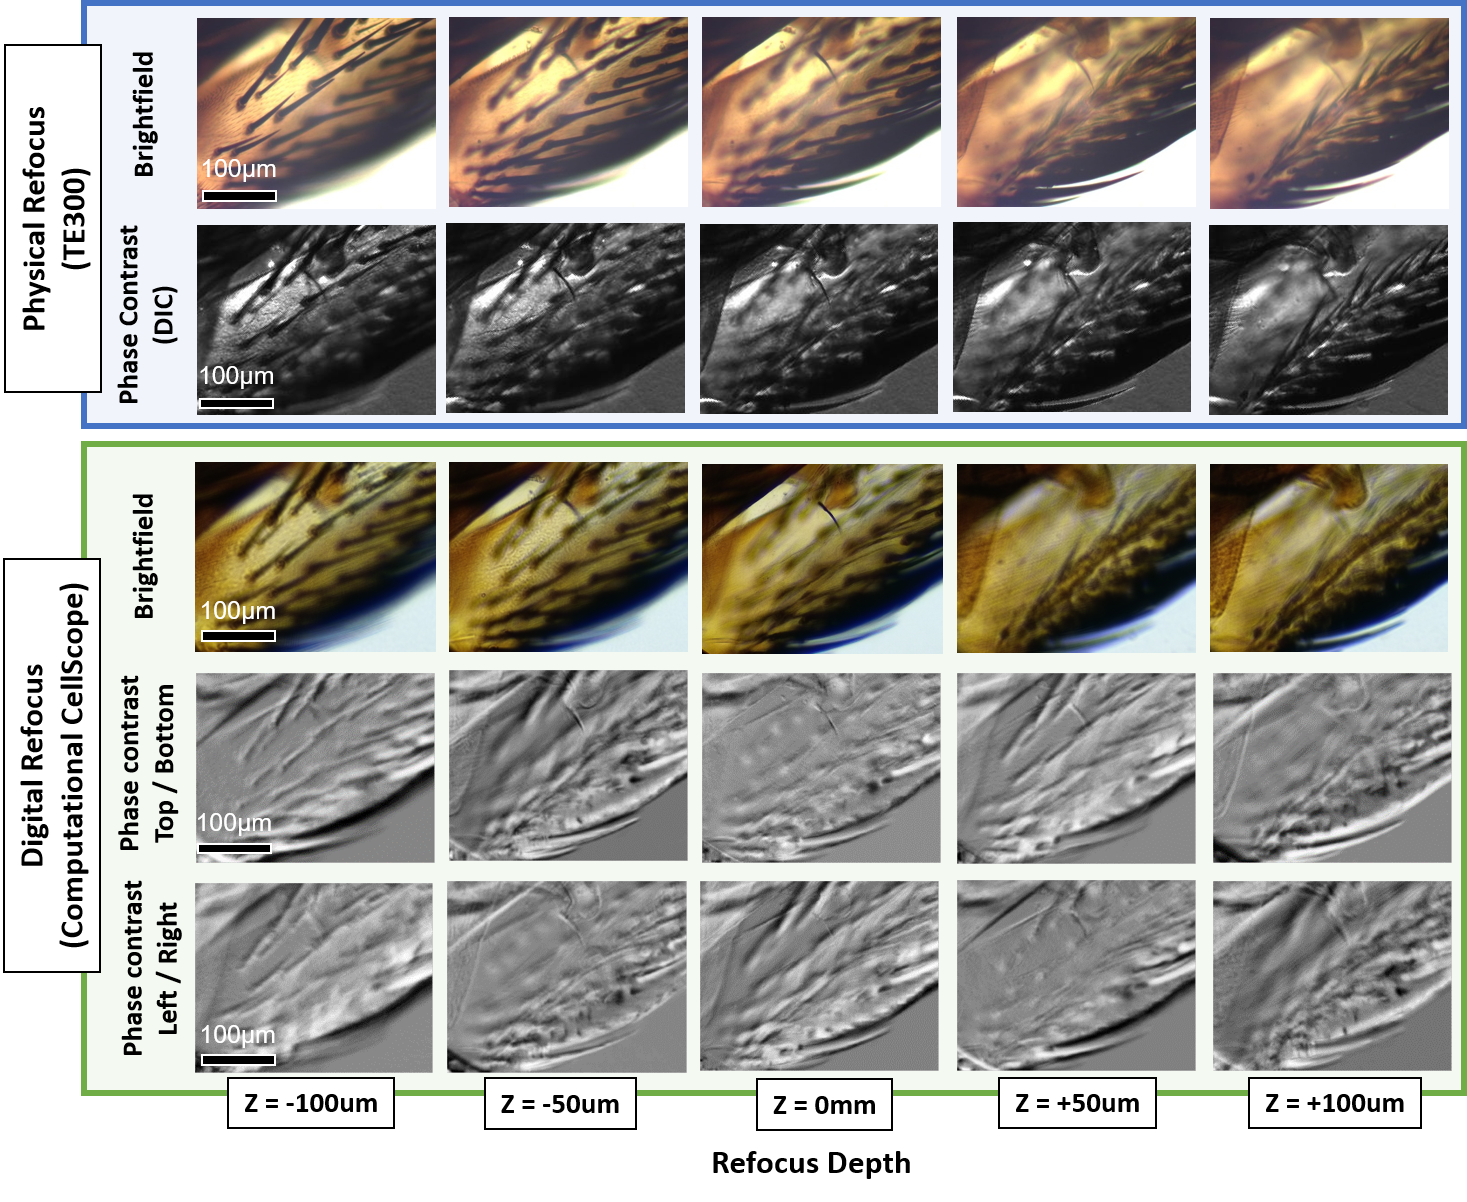
\includegraphics[width=\textwidth]{ccs-fig5.png}
\end{center}

\caption { {Digital refocusing on the Computational CellScope.} Comparison of digital refocusing to physical refocusing on a commercial microscope (Nikon TE300) of a house fly wing sample (AmScope PS200) with a 10$\times$ objective. Digitally refocused phase contrast images are also computed for both vertical and horizontal phase derivatives at different focus depths.} 

\label{fig:digrefocus}
\end{figure} 

Results are shown in Fig.~\ref{fig:digrefocus} for digitally refocused images as compared to physically refocused images on an inverted microscope (Nikon TE300), both with a 10$\times$ objective (0.25 NA). The phase contrast images show the first derivative of phase along both the vertical and horizontal directions, calculated from the same dataset using only the green color channel. The algorithm successfully refocused features across 400$\mu$m depth of field, limited by object thickness. Our refocusing achieves an axial resolution of approximately 5$\mu$m within $\pm50\mu$m of physical focus position, but degrades approximately linearly with increasing refocus distance~\cite{Tian14}. Processing time is approximately 1.5 minutes per depth slice for a 10$\times$ objective. 

\section{Hardware Implementation}
The illuminator consists of 4 major components: a hemispherical dome frame for mounting the LEDs, the LEDs themselves, controller circuit boards and the sample stage. The dome mounting structure is a rigid hemisphere designed to constrain the individual LEDs within an array of computationally positioned bores, aligning the LED with the radius vector to the sample center.  This hemisphere was designed with a $60\textrm{mm}$ radius in order to provide maximum intensity at the sample, given our desired number of LEDs and a minimum distance between neighboring LEDs. The part was 3D printed using a SLA printer (InterPro Models) to achieve the necessary 100$\mu$m printing resolution for accurate LED positioning. The LED angular positions were computed algorithmically to ensure uniform spacing across the dome, constrained by a minimum 150$\mu$m distance between bores for mechanical rigidity and a maximum angular separation of 3.85 degrees allowing for sufficient coherence area at the sample. This angular spacing means that 38 LEDs make up the brightfield region for our smallest NA objective (4$\times$), with even more for larger NA objectives, ensuring high quality digital refocusing results across a large range of depth slices for all objectives. The $3\textrm{mm}$ through-hole, white LEDs (Mouser 593-VAOL-3LWY4) were press fit into the dome and a rigid lateral constraint was provided by acrylic retaining inserts behind each individual LED. 508 of these LEDs were soldered directly to controller boards arranged above the array, with insulated leads to prevent electrical shorting.

Accounting for mechanical tolerances of the 3D printed dome and the LED epoxy lenses, manufacturing tolerances suggest that the maximum angular pointing error will be no greater than ±4.8 degrees. This corresponds to a maximum intensity attenuation of only 1.2\% due to assembly variation and tolerances across all illumination angles. Our illumination is also quite uniform across the field of view. The maximum field of view of our optical system has a radius of $1.25\textrm{mm}$, set by the eyepiece field-stop diameter of $10\textrm{mm}$ and assuming a 4$\times$ objective. Given the $60\textrm{mm}$ radius of curvature of our dome, this corresponds to illumination variation due to mechanical tolerances being less than 1\% across the field of view for each single LED illumination.  While this result is quite good, the spread of intensities between different LEDs is significantly larger (see Fig.~\ref{fig:dome}g), as a result of combined mechanical, electrical, and parts tolerances. Conveniently, a one-time calibration sweep of illumination angles, taken with no sample present, is sufficient to allow computational removal of this variation for all practical purposes.

The device used nine identical printed circuit boards placed in a fanned arrangement above the dome, each containing four LED controller chips (Texas Instruments TLC5926) serving up to 64 LEDs. These were controlled by a single Arduino Micro micro-controller, which calculates the appropriate bit pattern based on serial commands from an included Bluetooth transceiver. The array is fully addressable through a standard Bluetooth serial link; no wired connection to the phone is needed, although a powered USB connection is provided to charge the phone’s battery as well, for convenience. We operate the serial output at 115K baud and note that we can update the entire pattern with approximately 100ms latency, although we predefine some of the more complex LED illumination patterns and store them in the Arduino flash memory to further improve acquisition time. Thus our final acquisition time is primarily limited by the smartphone camera rather than the LED array control, so could be improved significantly with future smartphone releases.

The dome's power control board is tolerant of voltages between 7 and 20 VDC to allow compatibility with a large range of power sources, including a standard 12V automotive battery and a 100W wall-plug variable output power supply, as well as many commercially available portable power supplies for consumer electronics. During regular usage, the device requires no more than 2A of current, though it could potentially draw up to 4.8A of current when all LEDs are illuminated. This is not a typical use case, however, since simultaneous illumination inside and outside the objective NA amounts to an undesirable mixing of darkfield and brightfield contrast. Noting that for 4$\times$, 10$\times$, and 20$\times$ objective configurations there are more darkfield than brightfield LEDs, to reduce power consumption we perform darkfield illumination by default using an annulus with a width equivalent to 0.15NA rather than using all of the darkfield LEDs. This moderately reduces the contrast and resolution of darkfield images but significantly reduces power use during the darkfield illumination cycle. We note that the device can operate indefinitely without overheating issues for both multi-contrast and digital refocusing. 

% Application Timing and Screenshot figure
\begin{figure}
\begin{center}
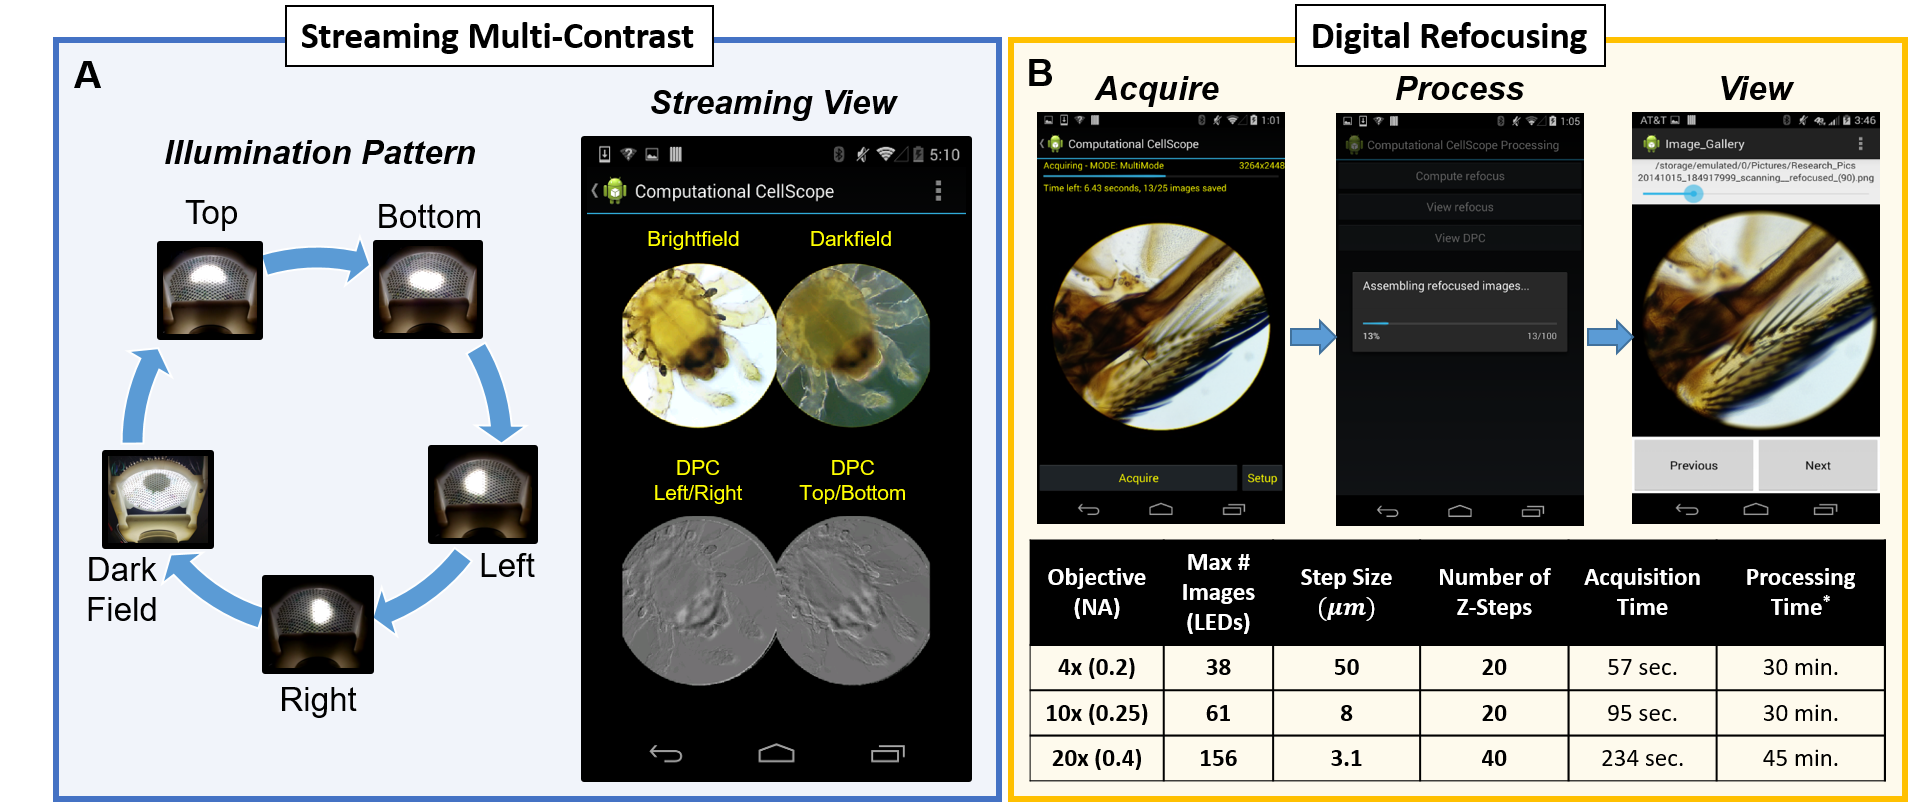
\includegraphics[width=\textwidth]{ccs-fig3.png}
\end{center}
\caption {{Android Application Workflow.} {a).} Schematic of streaming multi-contrast LED patterns. Here we vary the LED pattern in time and acquire and process images on the smartphone, producing a streaming multi-contrast display of a sample without any further post-processing. The user can touch any image to zoom in and stream an individual image. Total cycle time is 2.3 seconds.
{b).} Overview of workflow for digital refocusing mode. Table shows example processing and acquisition times for a typical dataset reconstruction. Axial Resolution is determined by the range of illumination angles sampled (defined by the objective NA). The number of z-steps were chosen such that refocus blur does not exceed 20 pixels. Processing and acquisition time can be reduced by selecting fewer refocus planes or by sparsely sampling LEDs, trading axial resolution for faster acquisition time.}
%, roughly ¼ the size of a typical 20 $\mu$m cell at 10$\times$

\label{fig:android}
\end{figure} 

\subsection{Acquisition Software and Processing}
It has previously been shown that using a smartphone as a microscope poses unique challenges intrinsic to the phone software~\cite{10.1371/journal.pone.0096906}. Smartphone cameras may only allow minimal quantitative control over standard imaging parameters (e.g. focus, exposure, gain), opting for opaque automatic algorithms that simplify the user experience. To circumvent these restrictions, we wrote a custom Android application that attempts to achieve the optimum imaging characteristics with our coded illumination configuration. In addition to a global tap-to-auto-focus capability, specific settings for each acquisition mode are detailed where appropriate in the following discussion. The software application also initiates and handles the Bluetooth connection to the domed array, enabling synchronized acquisition and array control through the standard Android API. Array control is thus transparent to the end-user, requiring them to simply pair the phone with the illuminator and press a connect button to initiate a Bluetooth connection. Our application was developed specifically for the Android platform, and will be compatible with any phone running Android OS version 4.0 or later. However, our algorithms were developed using the OpenCV Library, which is cross-platform for iOS (Apple, Inc.) and other operating systems. Thus most of our application code is portable to other smartphone platforms with moderate development effort. A screenshot of the acquisition and processing are shown in Fig.~\ref{fig:android}. The user may choose to collect and synthesize any or all of darkfield, refocused brightfield and DPC images.

In our application, images were acquired using the standard Android API, which does not provide an interface to set explicit exposure times in lieu of auto-exposure with predefined exposure offset values that are only effective while auto-exposure is active. To circumvent this issue, we included a short pre-illumination sequence before each dataset acquisition to lock exposure at the appropriate value. Additionally, to account for the asymmetric LED packing of our LED array, we choose equal numbers of LEDs for each half-circle used to form DPC images, since DPC requires symmetric and equal illumination. Finally, we incur significant latency between the camera shutter and the availability of the frame to our application within the API, due to post-processing algorithms integral to the phone and performed in the background (e.g. white balance and demosaicing). This severely limits our acquisition speeds, which will likely be improved in newer versions of Android that allow finer camera control through the API. Apple iOS offers a different camera API that may also offer improvements in acquisition speed.

Data post-processing was performed in a standalone Android app, where image stacks were loaded and processed on the phone. We employ a number of functions of the OpenCV Imaging library for Android to perform most of our computation. Individual DPC images are computed in less than a second, as demonstrated in our multi-contrast view mode. Digitally refocusing an image into 21 depth planes (±100 $\mu$m range with 10 $\mu$m sectioning) requires approximately 30 minutes of processing time, but the resulting 3D image stack can be interacted with in real-time; all other computational imaging results are much faster (~ 0.43 frames/sec). The long processing time is attributed to frequent loading and saving to the smartphone’s internal storage. We note that significant improvement in processing speeds for all of our algorithms is possible through implementation of our algorithms using the Android NDK, and is also expected as phone computational power increases with each product generation. These performance metrics were calculated on a Nexus 5 smartphone (LG Electronics) and may vary on other devices.




\chapter{Conclusion}
This thesis presents several computational imaging systems which use novel combinations of both hardware and software to image samples at high-speed, low cost, and in a portable system. Taken together, these methods illustrate the capabilities of a computational imaging system, and offer evidence of the impact these systems could have on the broader optical imaging community.

In Chapter 2, a single-shot method for quantitative phase and amplitude imaging which uses partially-coherent (angle-coded) multiplexed color illumination to recover the linearized optical field from a single deconvolution was presented. Our hardware requirements are simple, inexpensive, and compatible with most commercial microscopes through of the use of a color camera and a simple color filter insert placed at the back focal plane of the condenser lens, the same position as many removable phase contrast annulus rings. Unlike phase contrast and DIC, our method does not require special objectives or prisms, which reduces our hardware costs to that of the 3D printed filter itself. In addition, we can use our quantitative phase and amplitude methods to synthesize phase contrast and DIC images digitally, matching the functionality of existing phase imaging systems at a fraction of the cost.

In Chapter 3, a motion deblurring algorithm which uses time-coded active illumination to recover the complete optical field (phase and absorption) of a moving sample was presented. Our results show that by taking the OTF or WOTF of a system into account when designing blurring intensities, one can improve reconstruction quality of a deblurred image significantly. Further, we showed experimentally that motion deblur and quantitative phase retrieval can be applied together, and that our knowledge of the OTF improves reconstruction quality. This work did not consider non-linear kernels or unknown kernels, but the extension to this domain would be possible provided appropriate constraints were applied to the kernel shape and structure. An additional direction of interest is the blind deconvolution of motion kernels from a single blurred image. Since the WOTF inversion from a color image is over-determined, there is hope of recovering blur kernels using this over-determined information. A weakness of this method is in the need for precise alignment and synchronization of the stage, microscope, and illuminator. Blind deconvolution could account for small mis-alignments of the sample by solving for the blur kernel with little a-priori information.

In Chapter 4, a programmable domed LED array attachment and software for the CellScope mobile microscopy platform was demonstrated, enabling computational illumination techniques in a portable and affordable package. We demonstrated that this device allows multi-contrast imaging in near real-time, darkfield imaging without the cost or complexity of mechanical inserts, and phase imaging methods for label-free imaging of transparent cells and microorganisms in the field. Since our LED array is programmable, we are able to switch between contrast modes in real-time, simply by changing the illumination patterning. We currently stream at a frame rate of approximately 0.43 frames per second. Additionally, we use lightfield methods to enable digital refocusing of samples and have shown that this device is capable of refocusing samples across a 400$\mu$m range (at NA 0.25) with axial resolution of a few microns. All information needed to fabricate the Computational Cellscope dome, including the parts list, CAD designs, and software, are publicly available under the BSD open source license at: \begin{verbatim}www.laurawaller.com/OpenSource\end{verbatim}.

\section{Proposed Future Work}

In portable microscopy, future work will utilize similar LED array hardware, but add new imaging modes to our Computational CellScope device for quantitative 3D phase and super-resolution imaging. 3D imaging with tomographic inversions of both phase and amplitude information should be possible using similar datasets and more sophisticated algorithms~\cite{tian20153d}, if they can be adapted to mobile phone post-processing. One exciting potential extension of the device is to implement Fourier Ptychography~\cite{Zheng2013,Dong:14,Tian2014} or other super-resolution methods~\cite{Zhu2011,Greenbaum17122014} for achieving very wide field of view in conjunction with resolution well beyond the diffraction limit of the objective. These methods can also be combined with light field refocusing to obtain 3D stacks of both phase and intensity with large space-bandwidth product~\cite{tian20153d}. Our dome has been designed with these further applications in mind, so that these new capabilities can be added to our Computational CellScope platform as entirely software-side improvements. Thus, they may be deployed to existing devices via software updates over a cellular data network.

In addition, I hope to explore combinations of motion deblurring and portable microscopy for high-throughput imaging applications. Due to the calibration requirements of motion deblurring, it will be important to develop auto-calibration procedures to account for stage motion error and illumination mis-alignment to produce satisfactory images. This project can be formulated as a blind deconvolution problem, but I hope to incorporate non-linear terms into the calibration procedure to help improve results. In addition, I hope to combine these methods with high-throughput Fourier-Ptychographic methods in order to enable extreme high-throughput imaging, potentially into gigapixel scales.

\section{Acknowledgements}
I would like to thank Professor Laura Waller for providing careful guidance and support, especially during my first year in graduate school. I would also like to thank my entire lab for countless useless discussions. In addition, I would like to thank all professors, Post-Docs, graduate students, and undergraduate students at UC Berkeley who helped produce work which led to this thesis: Prof. Neil Switz, Prof. Daniel Fletcher, Prof. Lei Tian, Mike D’Ambrosio, Michael Chen, Jared Rulison, Hurshal Patel, Nitin Sadras, Aditya Gande, and Joel Whang.

\bibliographystyle{plos2009}
\bibliography{refscited}

\end{document}
